\documentclass[12pt,a4paper,oneside]{memoir}
\usepackage[T1]{fontenc}%necessario se si vuole il corretto funzionamento dell'algoritmo di costruzione dei capoversi
%pacchetto per la scelta dei font
\usepackage{cfr-lm}%Latin Modern esteso
\usepackage[utf8]{inputenc}%permette di inserire i caratteri nazionali
\usepackage[italian]{babel}
%impostazioni per l'italiano
\setISOcompliance
%\IntelligentComma
\usepackage{microtype}
\usepackage{parskip}
\frenchspacing
\setlength{\parindent}{0pt}
\usepackage{hyperref}
\usepackage{longtable}
\usepackage{array}
\usepackage{caption}
\usepackage[table,dvipsnames]{xcolor}
\definecolor{violetto}{RGB}{218,228,241}%prima riga tabelle
\definecolor{verdino}{RGB}{213,227,187}%colore box domande guida

% Don't forget to read the Memoir manual: memman.pdf

%%% Examples of Memoir customization
%%% enable, disable or adjust these as desired

%%% PAGE DIMENSIONS
% Set up the paper to be as close as possible to both A4 & letter:
\settrimmedsize{297mm}{210mm}{*}
\setlength{\trimtop}{0pt}
\setlength{\trimedge}{\stockwidth}
\addtolength{\trimedge}{-\paperwidth}
%\settypeblocksize{*}{\lxvchars}{1.618} % we want to the text block to have golden proportionals
%\setulmargins{50pt}{*}{*} % 50pt upper margins
%\setlrmargins{*}{*}{1.618} % golden ratio again for left/right margins
%\setheaderspaces{*}{*}{1.618}
\checkandfixthelayout 
%\settrimmedsize{297mm}{210mm}{*}
%\setlength{\trimtop}{0pt}
%\setlength{\trimedge}{\stockwidth}
%\addtolength{\trimedge}{-\paperwidth}
%\settypeblocksize{634pt}{448.13pt}{*}
%\setulmargins{4cm}{*}{*}
%\setlrmargins{*}{*}{1.5}
%\setmarginnotes{17pt}{51pt}{\onelineskip}
%\setheadfoot{\onelineskip}{2\onelineskip}
% This is from memman.pdf

%%% \maketitle CUSTOMISATION
% For more than trivial changes, you may as well do it yourself in a titlepage environment
%\pretitle{\begin{center}\sffamily\huge\MakeUppercase}
%\posttitle{\par\end{center}\vskip 0.5em}

%%% ToC (table of contents) APPEARANCE
\maxtocdepth{subsection} % include subsections
\renewcommand{\cftchapterpagefont}{}
\renewcommand{\cftchapterfont}{}     % no bold!

%%% HEADERS & FOOTERS
\pagestyle{ruled} % try also: empty , plain , headings , ruled , Ruled , companion

%%% CHAPTERS
\chapterstyle{hangnum} % try also: default , section , hangnum , companion , article, demo

\renewcommand{\chaptitlefont}{\Huge\sffamily\raggedright} % set sans serif chapter title font
\renewcommand{\chapnumfont}{\Huge\sffamily\raggedright} % set sans serif chapter number font

%%% SECTIONS
\hangsecnum % hang the section numbers into the margin to match \chapterstyle{hangnum}
\maxsecnumdepth{subsection} % number subsections

\setsecheadstyle{\Large\sffamily\raggedright} % set sans serif section font
\setsubsecheadstyle{\large\sffamily\raggedright} % set sans serif subsection font

%% END Memoir customization

\usepackage{calc}
\usepackage{multirow}%columns spanning several rows


%\title{Piano Triennale dell'Offerta Formativa dell'Istituto Comprensivo Statale ``Don Milani''}
%\author{}
%\date{27/10/2016} % Delete this line to display the current date

\makeatletter
\newcommand{\rmnum}[1]{\romannumeral #1}%numeri romani minuscoli
\newcommand{\Rmnum}[1]{\expandafter\@slowromancap\romannumeral #1@}%numeri romani maiuscoli
\makeatother

\usepackage{graphicx}
\usepackage{pdfpages}
\usepackage{epstopdf}
\DeclareGraphicsExtensions{.eps}


\newenvironment{elenco}{\begin{list}{$\bullet$}{%per gli elenchi puntati all'interno delle tabelle (P1, P2, ...)
              \setlength{\leftmargin}{4mm}%
              \setlength{\rightmargin}{1mm}%
               \setlength{\itemindent}{0mm}%             
               \setlength{\labelwidth}{2mm}%             
               \setlength{\labelsep}{2mm}%             
              \setlength{\itemsep}{-\parsep}%
              \setlength{\partopsep}{0pt}%
              \setlength{\topsep}{0pt}%
             \setlength{\parskip}{0pt}% 
              }}{\end{list}}
\newcolumntype{P}[1]{>{\endgraf\vspace*{-\baselineskip}}p{#1}}
%\usepackage[a-1b]{pdfx}%per generare un documento PDF/A
%%% BEGIN DOCUMENT
\begin{document}


\includepdf{copertina}

\clearpage



\chapter*{Premessa}

\begin{itemize}
\item Il presente Piano triennale dell'offerta formativa, relativo all'Istituto Comprensivo Statale ``Don Lorenzo Milani'' di Misterbianco (CT), è elaborato ai sensi di quanto previsto dalla legge 13 luglio 2015, n. 107, recante la ``Riforma del sistema nazionale di istruzione e formazione e delega per il riordino delle disposizioni legislative vigenti'';
\item il piano è stato elaborato dal collegio dei docenti sulla base degli indirizzi per le attività della scuola e delle scelte di gestione e di amministrazione definiti dal dirigente scolastico con proprio atto di indirizzo comunicato durante la seduta del Collegio dei docenti del 29/09/2015;
\item il piano ha ricevuto il parere favorevole del collegio dei docenti nella seduta del 18/01/2016;
\item il piano è stato approvato dal consiglio d'istituto nella seduta del 20/01/2016;
\item il piano, dopo l'approvazione, è stato inviato all'USR competente per le verifiche di legge ed in particolare per accertarne la compatibilità con i limiti di organico assegnato
\item il piano è stato aggiornato dal collegio dei docenti nella seduta del 26/10/2016;
\item il piano aggiornato è stato approvato dal consiglio d'istituto nella seduta del 27/10/2016.
\end{itemize}

\tableofcontents* % the asterisk means that the contents itself isn't put into the ToC

\chapter{Priorità strategiche}
Il presente Piano parte dalle risultanze dell'autovalutazione d'istituto, così come contenuta nel Rapporto di Autovalutazione (RAV), 
pubblicato sul sito web della scuola all'indirizzo:\\
\url{http://www.icsdonmilanimisterbianco.gov.it/}.\\

In particolare, si rimanda al RAV per quanto riguarda l'analisi del contesto in cui opera l'istituto, l'inventario delle risorse materiali, finanziarie, strumentali ed umane di cui si avvale, gli esiti documentati degli apprendimenti degli studenti, la descrizione dei processi organizzativi e didattici messi in atto.\\

Si riprendono qui in forma esplicita, come punto di partenza per la redazione del Piano, gli elementi conclusivi del RAV e cioè: priorità, traguardi di lungo periodo, obiettivi di processo.\\

\section{Priorità}
Le priorità si riferiscono agli obiettivi generali che la scuola si prefigge di realizzare nel lungo periodo attraverso l'azione di miglioramento. Le priorità che la scuola si pone devono necessariamente riguardare gli esiti degli studenti e, in questo ambito, il modello utilizzato per la stesura del RAV individua quattro aree obbligatorie --- risultati scolastici, risultati nelle prove standardizzate nazionali, competenze chiave e di cittadinanza, risultati a distanza --- e suggerisce di \textit{individuare un numero limitato di priorità (1 o 2) all'interno di una o due aree degli esiti degli studenti}.\\

Le priorità che l'Istituto si è assegnato per il prossimo triennio riguardano le seguenti aree:
\begin{enumerate}
\item Risultati nelle prove standardizzate nazionali;
\item Competenze chiave e di cittadinanza.
\label{priorità}
\end{enumerate}

\section{Traguardi di lungo periodo}
I traguardi di lungo periodo riguardano i risultati attesi in relazione alle priorità strategiche. Si tratta di risultati previsti a lungo termine (3 anni). Essi articolano in forma osservabile e/o misurabile i contenuti delle priorità e rappresentano le mete verso cui la scuola tende nella sua azione di miglioramento. Per ogni priorità individuata deve essere articolato il relativo traguardo di lungo periodo.\\

I traguardi che l'Istituto si è assegnato in relazione alle priorità sono:
\begin{enumerate}
\item Ridurre la percentuale di alunni della scuola primaria presenti nei primi due livelli del 5\%, rispetto al dato nazionale, sia per la matematica, che per l'italiano;
\item Ridurre la percentuale di alunni della scuola secondaria di I grado presenti nei primi due livelli del 5\%, rispetto al dato nazionale, sia per la matematica, che per l'italiano;
\item Riduzione delle note disciplinari, del sei in comportamento, dei consigli di classe straordinari, di episodi problematici.
\end{enumerate}

Le motivazioni della scelta effettuata sono le seguenti:
\begin{enumerate}
\item Uniformità dei risultati tra le classi parallele, soprattutto per quanto riguarda l'italiano (sia primaria che secondaria);
\item Per la scuola secondaria di primo grado, diminuire il numero degli alunni presenti nei primi due livelli, sia per la matematica che per l'italiano;
\item Promozione di competenze sociali: senso di legalità e di un'etica della responsabilità, collaborazione e lo spirito di gruppo.
\end{enumerate}

\section{Obiettivi di processo}
Gli obiettivi di processo rappresentano una definizione operativa delle attività su cui si intende agire concretamente per raggiungere le priorità strategiche individuate. Essi costituiscono degli obiettivi operativi da raggiungere nel breve periodo (un anno scolastico) e riguardano una o più aree di processo.\\

Gli obiettivi di processo che l'Istituto ha scelto di adottare in vista del raggiungimento dei traguardi sono:
\begin{enumerate}
\item Progettare percorsi per competenze;
\item Elaborare e somministrare prove standardizzate. Elaborare criteri di correzione comuni;
\item Potenziare l'uso delle tecnologie in classe;
\item Realizzare attività laboratoriali finalizzate alla differenziazione dei percorsi didattici per gli studenti con maggiori difficoltà;
\item Promozione della figura del docente tutor per supportare gli studenti in difficoltà.
\end{enumerate}

La progettazione di percorsi per competenze, il potenziamento delle tecnologie in classe, l'istituzione del docente tutor per supportare gli studenti in difficoltà,  sono alcune delle azioni che, operando a largo raggio, confluiscono sinergicamente al raggiungimento delle priorità.\\

Le prove e i relativi criteri comuni di correzione saranno uno strumento di valutazione oggettiva.\\

Le competenze sociali saranno promosse da attività laboratoriali e di gruppo, sia curricolari che non, per sviluppare negli alunni il senso di appartenenza alla comunità scolastica, e condividerne le regole e i codici di comportamento, contribuendo a migliorare le competenze di cittadinanza.\\

\section{Risultati delle prove Invalsi e scelte conseguenti}

\subsection[Terze classi della scuola secondaria]{Risultati delle terze classi della scuola secondaria di primo grado nell'ultimo triennio}
L'analisi dei risultati di apprendimento nelle prove standardizzate nazionali di Italiano e Matematica delle terze classi della scuola secondaria di primo grado (tabelle \ref{invalsi13-14-iii}, \ref{invalsi14-15-iii}, \ref{invalsi15-16-iii} e le figure \ref{fig:distr-italiano-iii}, \ref{fig:distr-matematica-iii}), ha messo in luce i seguenti punti di forza:
\begin{itemize}
\item un progressivo miglioramento dei risultati nella prova di Matematica;
\item la distribuzione degli alunni nei livelli di apprendimento\footnote{Sulla base dei risultati su scala nazionale, l'INVALSI ha costruito 5 livelli di apprendimento:\\
Livello 1 punteggio minore o uguale al 75\% della media nazionale;\\
Livello 2 punteggio maggiore del 75\% e minore o uguale del 95\% della media nazionale;\\
Livello 3 punteggio maggiore del 95\% e minore o uguale del 110\% della media nazionale;\\
Livello 4 punteggio maggiore del 110\% e minore o uguale del 125\% della media nazionale;\\
Livello 5 punteggio maggiore del 125\% della media nazionale.} in Matematica è andata migliorando, con una diminuzione del numero degli alunni presenti nei livelli 1 e 2 e un aumento nei livelli 3 e 5.
\end{itemize}
Per quanto riguarda i punti di debolezza:
\begin{itemize}
\item in Italiano il numero degli alunni nel livello di apprendimento più basso è andato aumentando, mentre il numero degli alunni nel livello di apprendimento più alto è andato diminuendo;
\item i risultati in Italiano sono, in tutti e tre gli anni, inferiori rispetto alla media italiana.
\end{itemize}

\begin{table}[htp]
\caption{Risultati classi terze scuola secondaria di primo gr. a.s. 2013/14.} \label{invalsi13-14-iii}
\footnotesize
\begin{tabular}{|p{1.5cm}|p{1cm}|p{1cm}|p{1cm}|p{1cm}|p{1cm}|p{1cm}|p{1cm}|p{1cm}|}\hline
%\multicolumn{9}{|c|}{Risultati classi terze scuola secondaria di primo gr. a.s. 2013/14}\\\hline
\rowcolor{violetto}
&\multicolumn{4}{c|}{italiano}&\multicolumn{4}{c|}{matematica}\\\hline
\rowcolor{violetto}
i\-sti\-tu\-to clas\-se&p. medio&sicilia&sud e isole&italia&p. medio&sicilia&sud e isole&italia\\\hline
&&
$54,0$&
$55,5$&
$61,4$&&
$50,7$&
$51,2$&
$57,3$\\\hline
i\-sti\-tu\-to&
$59,1$&
\centering{$\Uparrow$}&
\centering{$\Uparrow$}&
\centering{$\Downarrow$}&
$46,8$&
\centering{$\Downarrow$}&
\centering{$\Downarrow$}&
\centering{$\Downarrow$}\tabularnewline\hline
\Rmnum{3} A&
$59,3$&
\centering{$\Uparrow$}&
\centering{$\Uparrow$}&
\centering{$\Downarrow$}&
$48,8$&
\centering{$\Leftrightarrow$}&
\centering{$\Downarrow$}&
\centering{$\Downarrow$}\tabularnewline\hline
\Rmnum{3} B&
$64,1$&
\centering{$\Uparrow$}&
\centering{$\Uparrow$}&
\centering{$\Uparrow$}&
$54,6$&
\centering{$\Uparrow$}&
\centering{$\Uparrow$}&
\centering{$\Downarrow$}\tabularnewline\hline
\Rmnum{3} C&
$66,9$&
\centering{$\Uparrow$}&
\centering{$\Uparrow$}&
\centering{$\Uparrow$}&
$27,3$&
\centering{$\Downarrow$}&
\centering{$\Downarrow$}&
\centering{$\Downarrow$}\tabularnewline\hline
\Rmnum{3} D&
$50,1$&
\centering{$\Downarrow$}&
\centering{$\Downarrow$}&
\centering{$\Downarrow$}&
$52,9$&
\centering{$\Leftrightarrow$}&
\centering{$\Uparrow$}&
\centering{$\Downarrow$}\tabularnewline\hline
\end{tabular}
\end{table}


\begin{table}[htp]
\caption{Risultati classi terze scuola secondaria di primo gr. a.s. 2014/15.} \label{invalsi14-15-iii}
\footnotesize
\begin{tabular}{|p{1.5cm}|p{1cm}|p{1cm}|p{1cm}|p{1cm}|p{1cm}|p{1cm}|p{1cm}|p{1cm}|}\hline
%\multicolumn{9}{|c|}{Risultati classi terze scuola secondaria di primo gr. a.s. 2014/15}\\\hline
\rowcolor{violetto}
&\multicolumn{4}{c|}{italiano}&\multicolumn{4}{c|}{matematica}\\\hline
\rowcolor{violetto}
i\-sti\-tu\-to clas\-se&p. medio&sicilia&sud e isole&italia&p. medio&sicilia&sud e isole&italia\\\hline
&&$54,2$&$55,9$&$60,3$&&$46,9$&$48,2$&$53,5$\\\hline
i\-sti\-tu\-to&
$52,2$&
\centering{$\Leftrightarrow$}&
\centering{$\Downarrow$}&
\centering{$\Downarrow$}&
$53,8$&
\centering{$\Uparrow$}&
\centering{$\Uparrow$}&
\centering{$\Leftrightarrow$}\tabularnewline\hline
\Rmnum{3} A&
$48,0$&
\centering{$\Downarrow$}&
\centering{$\Downarrow$}&
\centering{$\Downarrow$}&
$52,3$&
\centering{$\Uparrow$}&
\centering{$\Uparrow$}&
\centering{$\Downarrow$}\tabularnewline\hline
\Rmnum{3} B&
$59,1$&
\centering{$\Uparrow$}&
\centering{$\Uparrow$}&
\centering{$\Downarrow$}&
$59,7$&
\centering{$\Uparrow$}&
\centering{$\Uparrow$}&
\centering{$\Uparrow$}\tabularnewline\hline
\Rmnum{3} C&
$49,6$&
\centering{$\Downarrow$}&
\centering{$\Downarrow$}&
\centering{$\Downarrow$}&
$55,1$&
\centering{$\Uparrow$}&
\centering{$\Uparrow$}&
\centering{$\Uparrow$}\tabularnewline\hline
\Rmnum{3} D&
$52,7$&
\centering{$\Leftrightarrow$}&
\centering{$\Downarrow$}&
\centering{$\Downarrow$}&
$47,5$&
\centering{$\Leftrightarrow$}&
\centering{$\Leftrightarrow$}&
\centering{$\Downarrow$}\tabularnewline\hline
\end{tabular}
\end{table}

\clearpage

\begin{table}[htp]
\caption{Risultati classi terze scuola secondaria di primo gr. a.s. 2015/16.} \label{invalsi15-16-iii}
\footnotesize
\begin{tabular}{|p{1.5cm}|p{1cm}|p{1cm}|p{1cm}|p{1cm}|p{1cm}|p{1cm}|p{1cm}|p{1cm}|}\hline
%\multicolumn{9}{|c|}{Risultati classi terze scuola secondaria di primo gr. a.s. 2015/16}\\\hline
\rowcolor{violetto}
&\multicolumn{4}{c|}{italiano}&\multicolumn{4}{c|}{matematica}\\\hline
\rowcolor{violetto}
i\-sti\-tu\-to clas\-se&p. medio&sicilia&sud e isole&italia&p. medio&sicilia&sud e isole&italia\\\hline
&&$51,0$&$52,5$&$57,6$&&$43,9$&$43,1$&$48,1$\\\hline
i\-sti\-tu\-to&
$51,3$&
\centering{$\Leftrightarrow$}&
\centering{$\Leftrightarrow$}&
\centering{$\Downarrow$}&
$51,3$&
\centering{$\Uparrow$}&
\centering{$\Uparrow$}&
\centering{$\Uparrow$}\tabularnewline\hline
\Rmnum{3} A&
$56,0$&
\centering{$\Uparrow$}&
\centering{$\Uparrow$}&
\centering{$\Downarrow$}&
$50,5$&
\centering{$\Uparrow$}&
\centering{$\Uparrow$}&
\centering{$\Uparrow$}\tabularnewline\hline
\Rmnum{3} B&$41,3$&
\centering{$\Downarrow$}&
\centering{$\Downarrow$}&
\centering{$\Downarrow$}&
$49,3$&
\centering{$\Uparrow$}&
\centering{$\Uparrow$}&
\centering{$\Uparrow$}\tabularnewline\hline
\Rmnum{3} C&
$55,5$&
\centering{$\Uparrow$}&
\centering{$\Uparrow$}&
\centering{$\Downarrow$}&
$53,9$&
\centering{$\Uparrow$}&
\centering{$\Uparrow$}&
\centering{$\Uparrow$}\tabularnewline\hline
\end{tabular}
\end{table}

\begin{figure}[htp]
\centering
\caption{Distribuzione degli alunni delle classi terze scuola secondaria di primo grado per livelli di apprendimento nel triennio nella prova di italiano.}
\label{fig:distr-italiano-iii}
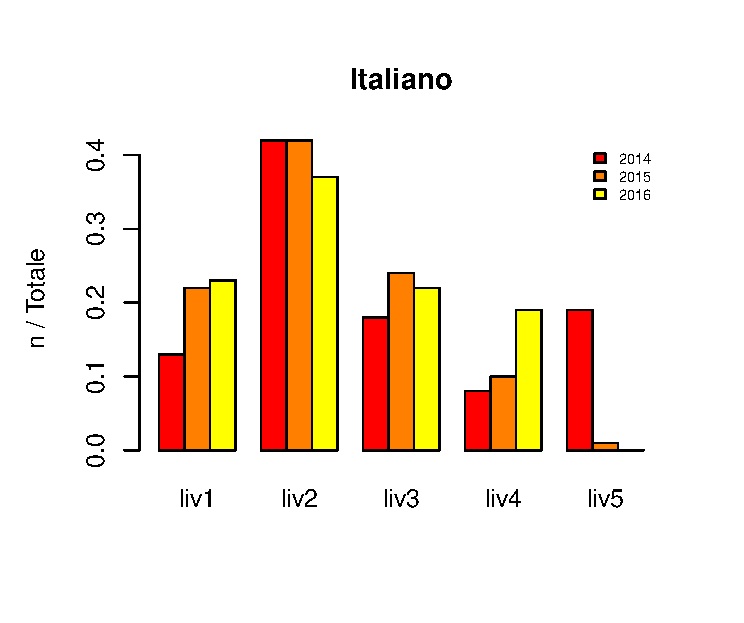
\includegraphics[width=0.8\linewidth]{italiano}
\end{figure}

\clearpage

\begin{figure}[htp]
\centering
\caption{Distribuzione degli alunni delle classi terze scuola secondaria di primo grado per livelli di apprendimento nel triennio nella prova di matematica.}
\label{fig:distr-matematica-iii}
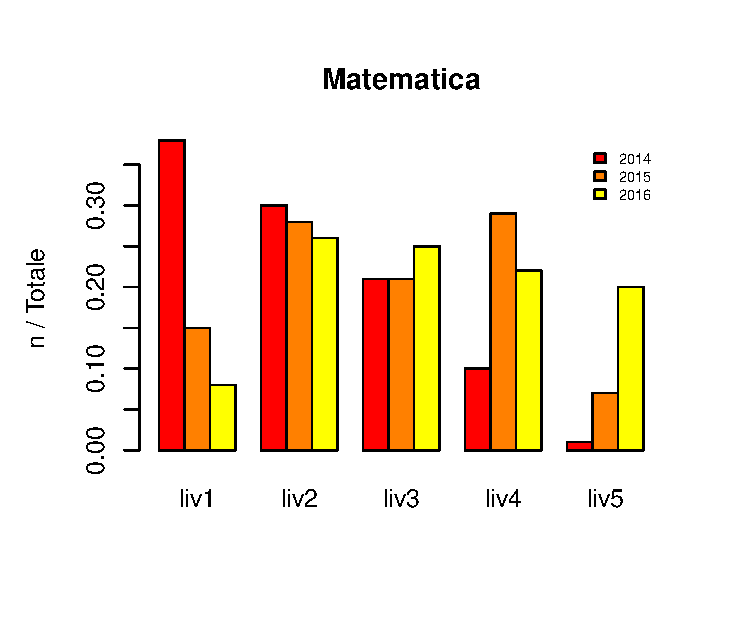
\includegraphics[width=0.8\linewidth]{matematica}
\end{figure}

\subsection[Seconde e quinte della scuola primaria]{Risultati delle seconde e delle quinte classi della scuola primaria nell'ultimo triennio}

I risultati relativi all'anno scolastico 2014/2015 non sono disponibili perché il numero degli alunni assenti alla prova ha superato il 50\% per ogni classe coinvolta nella prova. I risultati delle seconde relativi all'anno scolastico 2015/2016 non sono particolarmente significativi perché sono stati restituiti i dati di una sola classe su tre, a causa dell'elevato numero delle assenze.\\
L'analisi dei risultati di apprendimento nelle prove standardizzate nazionali di Italiano e Matematica delle seconde e quinte classi della scuola primaria (tabelle \ref{invalsi13-14-ii}, \ref{invalsi15-16-ii}, \ref{invalsi13-14-v} e \ref{invalsi15-16-v}), ha messo in luce i seguenti punti di forza:
\begin{itemize}
\item uniformità dei risultati tra le classi;
\item i risultati relativi all'anno scolastico 2013/2014 sono superiori anche alla media italiana.
\end{itemize}
Per quanto riguarda i punti di debolezza:
\begin{itemize}
\item per le quinte si nota una diminuzione dei punteggi dal 2013/2014 al 2015/2016 con risultati in quest'ultimo anno insufficienti rispetto alla media della Sicilia e anche relativamente a classi/scuole con background familiare simile;
\item per le quinte si nota una mancanza di uniformità nei risultati in Matamatica nell'anno scolastico 2015/2016;
\item i primi due livelli sono complessivamente più popolati rispetto alla media nazionale e di sud e isole sia per l'italiano  che per la matematica.
\end{itemize}

\`{E} opportuno precisare che una delle quattro classi quinte dell'anno scolastico 2015/2016, ha avuto un travagliato percorso didattico nei primi tre fondamentali anni della scuola primaria --- trasferimenti dei docenti, elevato numero di alunni svantaggiati, problematici e con scarse abilità di base --- tanto che si è operato un rimescolamento degli alunni delle sezioni A e B, tra il terzo ed il quarto anno. L'esito delle prove Invalsi, in particolare per la matematica, dimostra che non è stato possibile ridurre il divario con le altre classi, tuttavia dei miglioramenti sono stati riscontrati e, soprattutto, l'aver rilevato questa problematica, ha permesso di rivedere i criteri di formazione delle prime classi di ogni ciclo dal 2014/2015 in poi al fine di ridurre, quanto più possibile, la varianza tra le classi.  


\begin{table}[htp]
\caption{Risultati classi seconde scuola primaria gr. a.s. 2013/14.} \label{invalsi13-14-ii}
\footnotesize
\begin{tabular}{|p{1.5cm}|p{1cm}|p{1cm}|p{1cm}|p{1cm}|p{1cm}|p{1cm}|p{1cm}|p{1cm}|}\hline
%\multicolumn{9}{|c|}{Risultati classi seconde scuola primaria gr. a.s. 2013/14}\\\hline
\rowcolor{violetto}
&\multicolumn{4}{c|}{italiano}&\multicolumn{4}{c|}{matematica}\\\hline
\rowcolor{violetto}
i\-sti\-tu\-to clas\-se&p. medio&sicilia&sud e isole&italia&p. medio&sicilia&sud e isole&italia\\\hline
&&
$56,5$&
$58,3$&
$61,0$&&
$51,4$&
$53,1$&
$54,6$\\\hline
i\-sti\-tu\-to&
$75,7$&
\centering{$\Uparrow$}&
\centering{$\Uparrow$}&
\centering{$\Uparrow$}&
$66,5$&
\centering{$\Uparrow$}&
\centering{$\Uparrow$}&
\centering{$\Uparrow$}\tabularnewline\hline
\Rmnum{2} A&
$77,9$&
\centering{$\Uparrow$}&
\centering{$\Uparrow$}&
\centering{$\Uparrow$}&
$69,8$&
\centering{$\Uparrow$}&
\centering{$\Uparrow$}&
\centering{$\Uparrow$}\tabularnewline\hline
\Rmnum{2} B&
$74,0$&
\centering{$\Uparrow$}&
\centering{$\Uparrow$}&
\centering{$\Uparrow$}&
$55,7$&
\centering{$\Uparrow$}&
\centering{$\Uparrow$}&
\centering{$\Uparrow$}\tabularnewline\hline
\Rmnum{2} C&
$75,1$&
\centering{$\Uparrow$}&
\centering{$\Uparrow$}&
\centering{$\Uparrow$}&
$72,8$&
\centering{$\Uparrow$}&
\centering{$\Uparrow$}&
\centering{$\Uparrow$}\tabularnewline\hline
\end{tabular}
\end{table}

\begin{table}[htp]
\caption{Risultati classi seconde scuola primaria gr. a.s. 2015/16.} \label{invalsi15-16-ii}
\footnotesize
\begin{tabular}{|p{1.5cm}|p{1cm}|p{1cm}|p{1cm}|p{1cm}|p{1cm}|p{1cm}|p{1cm}|p{1cm}|}\hline
%\multicolumn{9}{|c|}{Risultati classi seconde scuola primaria gr. a.s. 2015/16}\\\hline
\rowcolor{violetto}
&\multicolumn{4}{c|}{italiano}&\multicolumn{4}{c|}{matematica}\\\hline
\rowcolor{violetto}
i\-sti\-tu\-to clas\-se&p. medio&sicilia&sud e isole&italia&p. medio&sicilia&sud e isole&italia\\\hline
&&
$44,9$&
$45,5$&
$48,2$&&
$48,7$&
$49,7$&
$51,0$\\\hline
i\-sti\-tu\-to&
$29,7$&
\centering{$\Downarrow$}&
\centering{$\Downarrow$}&
\centering{$\Downarrow$}&
$24,5$&
\centering{$\Downarrow$}&
\centering{$\Downarrow$}&
\centering{$\Downarrow$}\tabularnewline\hline
\Rmnum{2} A&
n.d.&
n.d.&
n.d.&
n.d.&
n.d.&
n.d.&
n.d.&
n.d.\tabularnewline\hline
\Rmnum{2} B&
$29,7$&
\centering{$\Downarrow$}&
\centering{$\Downarrow$}&
\centering{$\Downarrow$}&
$24,5$&
\centering{$\Downarrow$}&
\centering{$\Downarrow$}&
\centering{$\Downarrow$}\tabularnewline\hline
\Rmnum{2} C&
n.d.&
n.d.&
n.d.&
n.d.&
n.d.&
n.d.&
n.d.&
n.d.\tabularnewline\hline
\end{tabular}
\end{table}

\begin{table}[htp]
\caption{Risultati classi quinte scuola primaria gr. a.s. 2013/14.} \label{invalsi13-14-v}
\footnotesize
\begin{tabular}{|p{1.5cm}|p{1cm}|p{1cm}|p{1cm}|p{1cm}|p{1cm}|p{1cm}|p{1cm}|p{1cm}|}\hline
%\multicolumn{9}{|c|}{Risultati classi quinte scuola primaria gr. a.s. 2013/14}\\\hline
\rowcolor{violetto}
&\multicolumn{4}{c|}{italiano}&\multicolumn{4}{c|}{matematica}\\\hline
\rowcolor{violetto}
i\-sti\-tu\-to clas\-se&p. medio&sicilia&sud e isole&italia&p. medio&sicilia&sud e isole&italia\\\hline
&&
$53,9$&
$56,7$&
$61,0$&&
$56,7$&
$59,0$&
$62,9$\\\hline
i\-sti\-tu\-to&
$66,4$&
\centering{$\Uparrow$}&
\centering{$\Uparrow$}&
\centering{$\Uparrow$}&
$67,3$&
\centering{$\Uparrow$}&
\centering{$\Uparrow$}&
\centering{$\Uparrow$}\tabularnewline\hline
\Rmnum{5} A&
$62,7$&
\centering{$\Uparrow$}&
\centering{$\Uparrow$}&
\centering{$\Uparrow$}&
$63,0$&
\centering{$\Uparrow$}&
\centering{$\Uparrow$}&
\centering{$\Leftrightarrow$}\tabularnewline\hline
\Rmnum{5} B&
$69,6$&
\centering{$\Uparrow$}&
\centering{$\Uparrow$}&
\centering{$\Uparrow$}&
$60,4$&
\centering{$\Uparrow$}&
\centering{$\Leftrightarrow$}&
\centering{$\Downarrow$}\tabularnewline\hline
\Rmnum{5} C&
$68,6$&
\centering{$\Uparrow$}&
\centering{$\Uparrow$}&
\centering{$\Uparrow$}&
$78,1$&
\centering{$\Uparrow$}&
\centering{$\Uparrow$}&
\centering{$\Uparrow$}\tabularnewline\hline
\end{tabular}
\end{table}

\begin{table}[htp]
\caption{Risultati classi quinte scuola primaria gr. a.s. 2015/16.} \label{invalsi15-16-v}
\footnotesize
\begin{tabular}{|p{1.5cm}|p{1cm}|p{1cm}|p{1cm}|p{1cm}|p{1cm}|p{1cm}|p{1cm}|p{1cm}|}\hline
%\multicolumn{9}{|c|}{Risultati classi quinte scuola primaria gr. a.s. 2015/16}\\\hline
\rowcolor{violetto}
&\multicolumn{4}{c|}{italiano}&\multicolumn{4}{c|}{matematica}\\\hline
\rowcolor{violetto}
i\-sti\-tu\-to clas\-se&p. medio&sicilia&sud e isole&italia&p. medio&sicilia&sud e isole&italia\\\hline
&&
$57,8$&
$59,7$&
$63,5$&&
$45,7$&
$46,7$&
$51,0$\\\hline
i\-sti\-tu\-to&
$47,4$&
\centering{$\Downarrow$}&
\centering{$\Downarrow$}&
\centering{$\Downarrow$}&
$34,2$&
\centering{$\Downarrow$}&
\centering{$\Downarrow$}&
\centering{$\Downarrow$}\tabularnewline\hline
\Rmnum{5} A&
$56,3$&
\centering{$\Leftrightarrow$}&
\centering{$\Downarrow$}&
\centering{$\Downarrow$}&
$53,8$&
\centering{$\Uparrow$}&
\centering{$\Uparrow$}&
\centering{$\Uparrow$}\tabularnewline\hline
\Rmnum{5} B&
$40,2$&
\centering{$\Downarrow$}&
\centering{$\Downarrow$}&
\centering{$\Downarrow$}&
$24,1$&
\centering{$\Downarrow$}&
\centering{$\Downarrow$}&
\centering{$\Downarrow$}\tabularnewline\hline
\Rmnum{5} C&
$50,4$&
\centering{$\Downarrow$}&
\centering{$\Downarrow$}&
\centering{$\Downarrow$}&
$33,7$&
\centering{$\Downarrow$}&
\centering{$\Downarrow$}&
\centering{$\Downarrow$}\tabularnewline\hline
\Rmnum{5} D&
$44,0$&
\centering{$\Downarrow$}&
\centering{$\Downarrow$}&
\centering{$\Downarrow$}&
$32,7$&
\centering{$\Downarrow$}&
\centering{$\Downarrow$}&
\centering{$\Downarrow$}\tabularnewline\hline
\end{tabular}
\end{table}

\clearpage

\section{Scelte conseguenti}

%%%DA RIVEDERE COMPLETAMENTE

La mancanza/esiguità di fondi non ha consentito l'attivazione di corsi di recupero e di potenziamento extracurriculari , né il personale di potenziamento a disposizione ha potuto portare a termine quanto progettato  per il recupero e consolidamento delle abilità e delle conoscenze, in quanto spesso impegnato nella sostituzione dei docenti assenti (come previsto dalla L. 107). Le attività curriculari inerenti alla matematica del progetto  ``Con \ldots dividi''  hanno dato risultati positivi (come si evince dagli esiti Invalsi) , invece quelle inerenti all'italiano del progetto ``Il potere della parola'' hanno disatteso le aspettative , forse per la carenza di attività laboratoriali.

\section{Proposte e pareri provenienti dal territorio e dall'utenza}
Sono in corso continui contatti con gli altri istituti scolastici presenti nel territorio comunale e con l'ente locale per la realizzazione di alcuni interventi in particolare del settore relativo al diritto allo studio (educativa scolastica, finanziamento comodato d'uso libri di testo, interventi in genere relativi alla prevenzione del fenomeno della dispersione scolastica).


\chapter{Il Piano di Miglioramento}
Il Piano di Miglioramento si articola in 4 sezioni:
\begin{enumerate}
\item Scegliere gli obiettivi di processo più utili e necessari alla luce delle priorità individuate nella sezione 5 del RAV.
\item Decidere le azioni più opportune per raggiungere gli obiettivi scelti.
\item Pianificare gli obiettivi di processo individuati.
\item Valutare, condividere e diffondere i risultati alla luce del lavoro svolto dal Nucleo Interno di Valutazione.
\end{enumerate}
Le prime due sezioni permettono di documentare e condividere il percorso di problem solving messo in atto dalla scuola nella scelta degli obiettivi di processo e delle azioni di miglioramento ad essi connesse. Le sezioni 3 e 4, che costituiscono il cuore della progettazione del Piano di Miglioramento e del monitoraggio del suo andamento.

Ogni sezione è accompagnata da domande guida, utili per la compilazione del piano.


\section[Sezione 1. Scegliere gli obiettivi di processo]{Scegliere gli obiettivi di processo più rilevanti e necessari in tre passi (Sezione 1)}

Nella sezione 5 del RAV la scuola ha indicato alcuni obiettivi di processo che intende perseguire per raggiungere i traguardi connessi alle priorità. Per assicurarsi che la strada imboccata sia quella giusta la pianificazione del miglioramento riparte da qui: La scelta degli obiettivi è corretta? Sono questi gli obiettivi più utili alla promozione di un processo innovativo nella scuola? Sono connessi tra loro? E, soprattutto, la scuola si trova in condizioni oggettivamente favorevoli per la loro attuazione?


\subsection[Passo 1. Verificare la congruenza]{Verificare la congruenza tra obiettivi di processo e priorità/traguardi (Passo 1)}

Si chiede ora alla scuola di esplicitare la connessione tra ciascuno degli obiettivi di processo e le priorità individuate. Tale connessione deriva dal potenziale impatto che l'obiettivo potrà avere sul raggiungimento dei traguardi relativi alle priorità. In base a queste considerazioni, ogni obiettivo di processo può essere messo in relazione solo con una o con entrambe le priorità strategiche precedentemente identificate. In questo modo si ottiene un quadro sinottico degli obiettivi di processo, collegati alle priorità e ai traguardi.\\


\begin{center}
\fcolorbox{black}{verdino}{\hspace{5pt}%
\begin{minipage}[t]{.90\textwidth}

\vspace{1 em}

\textbf{Domande guida}\\

Ci sono nessi tra obiettivi e traguardi? se si, quali sono?\\
Ci sono ridondanze tra gli obiettivi individuati?\\
Gli obiettivi coprono tutti gli aspetti delle priorità dichiarate in modo efficace e completo?\\



\end{minipage}%
\hspace{5pt}
}
\end{center}


Nella Tabella \ref{obiettivi-e-priorità} vengono elencati gli obiettivi di processo, come indicati nella sezione 5 del RAV, e viene indicata con un ``SI'', nella colonna corrispondente al numero della priorità\footnote{Le due priorità sono state specificate a pagina \pageref{priorità}.} l'eventuale corrispondenza tra l'obiettivo e la priorità stessa.\\

\begin{table}[htp]
\caption{Relazione tra obiettivi di processo e priorità strategiche. Elencare gli obiettivi di processo come indicati nella sezione 5 del RAV e barrare le colonne 1 e/o 2 per indicare l'attinenza di ciascuno a una o entrambe le priorità.}  \label{obiettivi-e-priorità}
\footnotesize
\begin{tabular}{|>{\raggedright}p{4.cm}|>{\raggedright}p{5.9cm}|>{\raggedright}p{0.975cm}|>{\raggedright\arraybackslash}p{0.975cm}|}
\hline
\rowcolor{violetto}
Area di processo&Obiettivi di processo&\multicolumn{2}{c|}{Priorità \ldots}\\\cline{3-4}
\rowcolor{violetto}
&&1&2\\\hline
Curricolo, progettazione e valutazione&1 Progettare percorsi per competenze.&SI&\\\cline{2-4}
&2 Elaborare e somministrare prove standardizzate. Elaborare criteri di correzione comuni.&SI&\\\hline
Ambiente di apprendimento&1 Potenziare l'uso delle tecnologie in classe.&SI&\\\cline{2-4}
&2&&\\\hline
Inclusione e differenziazione&1 Realizzare attività laboratoriali finalizzate alla differenziazione dei percorsi didattici per gli studenti con maggiori difficoltà.&SI&SI\\\cline{2-4}
&2 Promuovere una figura di docente tutor per supportare gli studenti in difficoltà.&SI&\\\hline
\multirow{2}{35mm}{Continuità e orientamento}&1&&\\\cline{2-4}
&2&&\\\hline
Orientamento strategico e organizzazione della scuola&1 Revisione dei compiti affidati al personale docente, con particolare riferimento ai docenti coordinatori di classe.&&\\\cline{2-4}
&2&&\\\hline
Sviluppo e valorizzazione delle risorse umane&1 Aumentare la partecipazione dei docenti alle iniziative di formazione.&SI&SI\\\cline{2-4}
&2 Migliorare le ricadute delle attività di formazione nell'attività ordinaria della scuola.&SI&SI\\\hline
\multirow{2}{35mm}[3mm]{Integrazione con il territorio e rapporti con le famiglie}&\raisebox{1.6ex}[0cm][0cm]{1} \rule{0em}{3.5ex}&&\\\cline{2-4}
&\raisebox{1.6ex}[0cm][0cm]{2} \rule{0em}{3.5ex}&&\\\hline
\end{tabular}
\end{table}

\clearpage

\subsection[Passo 2. Elaborare una scala di rilevanza degli obiettivi di processo]{Elaborare una scala di rilevanza degli obiettivi di processo (Passo 2)}
Al fine di valutare la rilevanza di ciascuno degli obiettivi di processo, è importante compiere una stima della loro fattibilità. Ad ogni obiettivo si attribuisce un valore di fattibilità e uno di impatto, determinando una scala di rilevanza.\\

La stima dell'impatto implica una valutazione degli effetti che si pensa possano avere le azioni messe in atto al fine perseguire l'obiettivo descritto.\\

La stima della fattibilità si attua sulla base di una valutazione delle reali possibilità di realizzare le azioni previste, tenendo conto delle risorse umane e finanziarie a disposizione.\\

Si possono considerare i punteggi da 1 a 5 come segue:\\
1= nullo\\
2= poco\\
3= abbastanza\\
4= molto\\
5= del tutto\\

Il prodotto dei due valori fornisce una scala di rilevanza degli obiettivi di processo da mettere in atto.\\

Alla luce di queste valutazioni, la scuola può analizzare con più attenzione il peso strategico degli obiettivi di processo, in vista della pianificazione delle azioni ad essi sottese. In base ai risultati ottenuti la scuola può valutare se rivedere gli obiettivi dichiarati nel RAV, concentrandosi su quelli di rilevanza maggiore e, all'occorrenza, eliminare o ridimensionare il peso degli obiettivi di minore rilevanza.\\


\begin{center}
\fcolorbox{black}{verdino}{\hspace{5pt}%
\begin{minipage}[t]{.90\textwidth}

\vspace{1 em}

\textbf{Domande guida}\\

Ci sono obiettivi che, sebbene siano importanti, non è possibile realizzare?\\
Su quali obiettivi è opportuno concentrare le risorse a disposizione?\\



\end{minipage}%
\hspace{5pt}
}
\end{center}

\begin{table}[htp]
\caption{Calcolo della necessità dell'intervento sulla base di fattibilità ed impatto. Al fine di calcolare la rilevanza dell'obiettivo utilizzare la tabella riportando le stime sulla fattibilità e sull'impatto e il prodotto dei due valori numerici.}  \label{fattibilità-impatto-intervento}
\footnotesize
\begin{tabular}{|>{\raggedright}p{.67cm}|>{\raggedright}p{5.67cm}|>{\raggedright}p{1.195cm}|>{\raggedright}p{1.195cm}|>{\raggedright\arraybackslash}p{2.52cm}|}
\hline
\rowcolor{violetto}
&Obiettivo di processo elencati&Fat\-ti\-bi\-li\-tà (da 1 a 5)&Impatto (da 1 a 5)&Prodotto: valore che identifica la rilevanza dell'intervento\\\hline
1&Progettare percorsi per competenze.&4&4&16\\\hline
2&Elaborare e somministrare prove standardizzate. Elaborare criteri di correzione comuni.&4&4&16\\\hline
3&Potenziare l'uso delle tecnologie in classe.&4&4&16\\\hline
4&Realizzare attività laboratoriali finalizzate alla differenziazione dei percorsi didattici per gli studenti con maggiori difficoltà.&3&4&12\\\hline
5&Promuovere una figura di docente tutor per supportare gli studenti in difficoltà.&1&4&4\\\hline
6&Revisione dei compiti affidati al personale docente, con particolare riferimento ai docenti coordinatori di classe.&4&4&16\\\hline
7&Aumentare la partecipazione dei docenti alle iniziative di formazione.&2&4&8\\\hline
8&Migliorare le ricadute delle attività di formazione nell'attività ordinaria della scuola.&2&4&8\\\hline
\end{tabular}
\end{table}


\subsection[Passo 3. Ridefinire l'elenco degli obiettivi di processo e indicare i risultati attesi]{Ridefinire l'elenco degli obiettivi di processo e indicare i risultati attesi, gli indicatori di monitoraggio del processo e le modalità di misurazione dei risultati (Passo 3)}

Sulla base del lavoro precedente, la scuola può definire una lista ordinata degli obiettivi di processo, che saranno oggetto della successiva pianificazione.\\
Per ciascun obiettivo è necessaria una chiara definizione dei risultati attesi e degli indicatori su cui basare la misurazione periodica dei processi attivati, ai fini del monitoraggio dell'efficacia delle azioni intraprese. I risultati attesi e gli indicatori di processo devono essere espressi in una forma concreta e osservabile e saranno recuperati al momento del monitoraggio delle singole azioni.\\


\begin{center}
\fcolorbox{black}{verdino}{\hspace{5pt}%
\begin{minipage}[t]{.90\textwidth}

\vspace{1 em}

\textbf{Domande guida}\\

Quali sono gli obiettivi che s'intendono raggiungere nel prossimo anno scolastico?\\
Quali risultati ci si attende da ciascun obiettivo di processo scelto?\\
Quali indicatori dovranno essere utilizzati per capire se quella che si sta seguendo è la giusta direzione, al fine di raggiungere gli obiettivi previsti? In che modo  saranno misurati?\\



\end{minipage}%
\hspace{5pt}
}
\end{center}

\begin{footnotesize}
\captionsetup{width=13.5cm}
\begin{longtable}{|>{\raggedright}p{.342cm}|>{\raggedright}p{2.727cm}|>{\raggedright}p{2.727cm}|>{\raggedright}p{2.727cm}|>{\raggedright\arraybackslash}p{2.727cm}|}
\caption{Risultati attesi e  monitoraggio. Nella colonna ``indicatori di monitoraggio'' esprimere un elemento su cui basare il controllo periodico del processo in atto. L'indicatore dovrebbe essere un valore misurabile o comunque accertabile in modo univoco.} \label{risultati-e-monitoraggio}\\
\hline
\rowcolor{violetto}
&Obiettivo di processo in via di attuazione&Risultati attesi&Indicatori di monitoraggio&Modalità di rilevazione\\ \hline
\endfirsthead
\hline
\rowcolor{violetto}
&Obiettivo di processo in via di attuazione&Risultati attesi&Indicatori di monitoraggio&Modalità di rilevazione\\ \hline
\endhead
\hline \multicolumn{5}{r}{\emph{Continua nella pagina successiva}}
\endfoot
\hline
\endlastfoot
1&``Il potere della parola: evoluzione del lessico''.&Il miglioramento nella lettura, nella comprensione del testo, nella comunicazione orale, nella produzione scritta, nel lessico e nella metalinguistica.&Diminuire il numero di allievi nelle fasce L1 – L2 ($-5\%$: Dati INVALSI 2015-2016 sia per la scuola primaria che per la secondaria di I grado). 
Aumentare il numero di alunni nelle fasce L4 – L5 ($+5\%$: Dati INVALSI 2015-2016 sia per la scuola primaria che per la secondaria di $1^{\circ}$ grado).
Ridurre il numero di allievi gravemente&Raccolta dati sulla ricaduta delle azioni, da valutare in sede dipartimentale e di consiglio di classe (in itinere e finale);
somministrazione test di gradimento agli studenti e alle famiglie; somministrazione di prove comuni oggettive e criteri di correzione comuni; valutazione dei risultati delle prove invalsi.\\ \hline
&&&insufficienti al primo quadrimestre: $-25\%$.
Risultati delle prove INVALSI in italiano con un miglioramento degli esiti del $5\%$ nella differenza tra il risultato della scuola e la media nazionale e delle scuole con background simile. Somministrazione periodica di prove per classi parallele.&\\ \hline
2&``Con \ldots dividi''&Promuovere esperienze significative in cui gli strumenti matematici si mostrano sempre più utili per operare nella realtà.
Formulare ipotesi, controllare le conseguenze, progettare e sperimentare, discutere e argomentare le proprie scelte, raccogliere dati e costruire significati.&Diminuire il numero di allievi nelle fascia L2 ($-5\%$: Dati INVALSI 2015-16 solo per la prova Nazionale).
Diminuire il numero di allievi nelle fascia L1 ($-5\%$: Dati INVALSI 2015-16 scuola primaria).
Aumentare il numero di alunni nelle fasce L4 – L5 ($+5\%$: Dati INVALSI 2015-16 per la scuola primaria).&Raccolta dati sulla ricaduta delle azioni, da valutare in sede dipartimentale e di consiglio di classe (in itinere e finale); somministrazione test di gradimento agli studenti e alle famiglie; somministrazione di prove comuni oggettive e criteri di correzione comuni; valutazione dei risultati delle prove invalsi.\\ \hline
&&&Aumentare il numero di allievi nelle fascia L5 ($+5\%$: Dati INVALSI 2015-16 solo per la prova Nazionale).
Ridurre il numero di allievi gravemente insufficienti al primo quadrimestre : $-25\%$.
Risultati delle prove INVALSI in matematica con un miglioramento degli esiti nella scuola primaria del $5\%$ nella differenza tra il risultato della scuola e la media nazionale e un mantenimento della percentuale superiore nella Prova Nazionale.&\\ \hline
3&Coro, propedeutica musicale, nella scuola primaria&Allestimento di eventi canori e musicali, condivisione di regole e capacità di lavoro in gruppo&Riduzione delle assenze, degli ingressi in ritardo, delle note disciplinari, dei sei in comportamento, aumento del numero delle iscrizioni nell'indirizzo musicale.&Raccolta dati sulla ricaduta delle azioni, da valutare in sede di consiglio di classe (in itinere e finale);
somministrazione test di gradimento agli studenti e alle famiglie.\\ \hline
4&Formazione&Diffondere maggiormente la didattica laboratoriale riducendo i tempi della lezione frontale.
Incentivare l'uso delle nuove tecnologie in ambito didattico.&Incremento dell'uso della LIM nella didattica quotidiana (\mbox{$>1$} lezione settimanale).
Incremento dei docenti che sperimentano in aula le tecniche e gli strumenti suggeriti durante la formazione ($\ge50\%$).
Motivare l'apprendimento degli alunni attraverso l'uso delle nuove tecnologie legate alla didattica ($\ge50\%$ delle risposte positive al questionario).
Decremento delle insufficienze e delle gravi insufficienze: confronto con le prove in itinere durante il $2^{\circ}$ quadrimestre ($-25\%$).&Utilizzo delle piattaforme e-learning presenti nel sito della scuola, per la condivisione di materiale didattico da mettere a disposizione di tutti i docenti.
Raccolta dati sulla ricaduta indiretta delle azioni da valutare in sede dipartimentale e di consiglio di classe (in itinere e finale).
Somministrazione test di gradimento ai docenti in formazione e agli studenti.\\ \hline
\end{longtable}
\end{footnotesize}

\section[Sezione 2. Azioni per raggiungere ciascun obiettivo]{Decidere le azioni per raggiungere ciascun obiettivo di processo in due passi (Sezione 2)}

\subsection[Passo 1. Ipotizzare le azioni da compiere]{Ipotizzare le azioni da compiere considerandone i possibili effetti negativi e positivi a medio e a lungo termine (Passo 1)}

Decidere le azioni da compiere è un passaggio che richiede una riflessione attenta in termini di valutazione delle potenziali opportunità e rischi.\\
Occorre considerare che le azioni che si intraprenderanno potranno avere degli effetti positivi ma anche potenziali ricadute negative su altre dimensioni o attività nelle quali la scuola è impegnata.\\
è opportuno inoltre tenere presente che gli effetti delle azioni intraprese non si esauriranno nel breve periodo, ma avranno anche effetti di medio e lungo periodo.\\


\begin{center}
\fcolorbox{black}{verdino}{\hspace{5pt}%
\begin{minipage}[t]{.90\textwidth}

\vspace{1 em}

\textbf{Domande guida}\\

Quali sono gli effetti positivi che un'azione può produrre all'interno della scuola?\\
Quali sono invece gli aspetti negativi che la stessa azione può produrre, innescando meccanismi non virtuosi?\\
Queste azioni produrranno effetti anche i nei prossimi anni?\\


\end{minipage}%
\hspace{5pt}
}
\end{center}

\begin{table}[htp]
\caption{Valutazione degli effetti positivi e negativi delle azioni.}  \label{valutazioni-effetti-azioni}
\footnotesize
\begin{tabular}{|>{\raggedright}p{1.902cm}|>{\raggedright}p{2.337cm}|>{\raggedright}p{2.337cm}|>{\raggedright}p{2.337cm}|>{\raggedright\arraybackslash}p{2.337cm}|}
\hline
\rowcolor{violetto}
Azione prevista&Effetti positivi all'interno della scuola a medio termine&Effetti negativi all'interno della scuola a medio termine&Effetti positivi all'interno della scuola a lungo termine&Effetti negativi all'interno della scuola a lungo termine\\ \hline
1&con\-so\-li\-da\-men\-to delle capacità di comprensione e di rielaborazione del testo.&&Mi\-glio\-ra\-men\-to degli esiti scolastici e nelle prove INVALSI.&\\ \hline
2&Tradurre le situazioni reali in termini matematici e riconoscere gli schemi ricorrenti.&&Mi\-glio\-ra\-men\-to degli esiti scolastici e nelle prove INVALSI.&\\ \hline
3&Maggiore partecipazione alle attività scolastiche, diminuzione delle assenze.&&Maggiore motivazione all'apprendimento.&\\ \hline
4&Incremento dell'uso della LIM, sperimentazione di metodologie didattiche innovative.&&Maggiore motivazione degli alunni all'apprendimento.&\\ \hline	
\end{tabular}
\end{table}

\clearpage

\subsection[Passo 2. Rapportare gli effetti a un quadro di riferimento innovativo]{Rapportare gli effetti delle azioni a un quadro di riferimento innovativo (Passo 2)}

Le azioni pianificate avranno effetti duraturi se incideranno sul raggiungimento di obiettivi a breve termine, ma soprattutto se rappresenteranno un'occasione per avviare un profondo processo di innovazione e cambiamento della scuola.\\

Le azioni che s'intendono attivare vengono quindi messe in relazione con il quadro di riferimento che emerge dal lavoro che INDIRE svolge con le scuole delle Avanguardie Educative e si collega fortemente a quanto previsto dalla Legge 107/15 nota come ``Buona Scuola''.\\


\begin{center}
\fcolorbox{black}{verdino}{\hspace{5pt}%
\begin{minipage}[t]{.90\textwidth}

\vspace{1 em}

\textbf{Domande guida}\\

Le azioni possono essere connesse a qualcuno degli obiettivi previsti dalla Legge 107/15?\\
Le azioni prevedono modifiche agli ambienti di apprendimento e/o all'organizzazione scolastica?\\
Nelle azioni descritte si può riconoscere una linea di tendenza che porta verso l'innovazione?\\


\end{minipage}%
\hspace{5pt}
}
\end{center}

\begin{table}[htp]
\caption{Caratteri innovativi.}  \label{caratteri-innovativi}
\footnotesize
\begin{tabular}{|>{\raggedright}p{6.2572cm}|>{\raggedright\arraybackslash}p{6.2572cm}|}
\hline
\rowcolor{violetto}
Caratteri innovativi dell'obiettivo&Connessione con il quadro di riferimento di cui in Appendice A e B\\ \hline
1. Adeguamento dei codici comunicativi dei giovani ai differenti contesti: formale, non formale e informale&comma 7, lettera a) e p)\\ \hline
2. Verticalizzazione dell'attività laboratoriale&comma 7, lettera b) e p)\\ \hline
3. Arricchimento delle attività performative dell'orchestra dell'istituto&comma 7, lettera c)\\ \hline
4. La formazione dei docenti consentirà l'uso di metodologie didattiche tali da sollecitare la partecipazione attiva degli alunni nella costruzione del sapere e nella acquisizione delle competenze&comma 124 e punto n. 2 del Manifesto del movimento delle Avanguardie Educative (Sfruttare le opportunità offerte dalle ICT e dai linguaggi digitali per supportare nuovi modi di insegnare, apprendere e valutare)\\ \hline
\end{tabular}
\end{table}

\section[Sezione 3. Pianificare le azioni di ciascun obiettivo]{Pianificare le azioni di ciascun obiettivo di processo individuato in tre passi (Sezione 3)}

\subsection[Passo 1. Definire l'impegno delle risorse umane e strumentali]{Definire l'impegno delle risorse umane e strumentali (Passo 1)}

La pianificazione delle azioni è il cuore della predisposizione del piano. Si parte con la previsione dell'impegno di risorse umane interne alla scuola, definendo ciò che esula dalle normali funzioni di servizio e che ha un impatto aggiuntivo di carattere finanziario (docenti, personale ATA, DS) e di quelle esterne (consulenti, formatori, ecc.), quantificando le spese che la scuola intende sostenere per l'attuazione delle azioni descritte.\\

\begin{center}
\fcolorbox{black}{verdino}{\hspace{5pt}%
\begin{minipage}[t]{.90\textwidth}

\vspace{1 em}

\textbf{Domande guida}\\

Quali sono le risorse umane interne che la scuola ha a disposizione per raggiungere gli obiettivi di processo?\\
Quali sono le risorse umane esterne necessarie ad attivare i processi in modo efficace?\\
Quali sono le fonti finanziarie da cui la scuola intende attingere per coprire le spese necessarie?\\



\end{minipage}%
\hspace{5pt}
}
\end{center} 

\begin{table}[htp]
\caption{Descrivere l'impegno di risorse umane interne alla scuola.}  \label{descrivere-impegno-interno}
Obiettivo 1\\


\footnotesize
\begin{tabular}{|>{\raggedright}p{2.249851cm}|>{\raggedright}p{2.249851cm}|>{\raggedright}p{2.249851cm}|>{\raggedright}p{2.249851cm}|>{\raggedright\arraybackslash}p{2.249851cm}|}
\hline
\rowcolor{violetto}
Figure professionali&Tipologia di attività&Ore aggiuntive presunte&Costo previsto&Fonte finanziaria\\\hline
Docenti interni&Attività curricolare&Nessuna&$0,00$&\\\hline
Personale ATA&Attività curricolare&Nessuna&$0,00$&\\\hline
Altre figure&Nessuna&Nessuna&$0,00$&\\\hline
\multicolumn{5}{r}{\emph{Continua nella pagina successiva}}\\
\end{tabular}
\end{table}
\begin{table}[htp]
\normalsize{Obiettivo 2}\\

\footnotesize
\begin{tabular}{|>{\raggedright}p{2.249851cm}|>{\raggedright}p{2.249851cm}|>{\raggedright}p{2.249851cm}|>{\raggedright}p{2.249851cm}|>{\raggedright\arraybackslash}p{2.249851cm}|}\hline
\rowcolor{violetto}
Figure professionali&Tipologia di attività&Ore aggiuntive presunte&Costo previsto&Fonte finanziaria\\\hline
Docenti interni&Attività curricolare&Nessuna&$0,00$&\\\hline
Personale ATA&Attività curricolare&Nessuna&$0,00$&\\\hline
Altre figure&Nessuna&Nessuna&$0,00$&\\\hline
\end{tabular}

\vspace{1em}

\normalsize{Obiettivo 3}\\

\footnotesize
\begin{tabular}{|>{\raggedright}p{2.249851cm}|>{\raggedright}p{2.249851cm}|>{\raggedright}p{2.249851cm}|>{\raggedright}p{2.249851cm}|>{\raggedright\arraybackslash}p{2.249851cm}|}\hline
\rowcolor{violetto}
Figure professionali&Tipologia di attività&Ore aggiuntive presunte&Costo previsto&Fonte finanziaria\\\hline
Docenti interni&Attività curricolare&Nessuna&$0,00$&\\\hline
Personale ATA&Attività curricolare&Nessuna&$0,00$&\\\hline
Altre figure&Nessuna&Nessuna&$0,00$&\\\hline
\end{tabular}

\vspace{1em}

\normalsize{Obiettivo 4}\\

\footnotesize
\begin{tabular}{|>{\raggedright}p{2.249851cm}|>{\raggedright}p{2.249851cm}|>{\raggedright}p{2.249851cm}|>{\raggedright}p{2.249851cm}|>{\raggedright\arraybackslash}p{2.249851cm}|}\hline
\rowcolor{violetto}
Figure professionali&Tipologia di attività&Ore aggiuntive presunte&Costo previsto&Fonte finanziaria\\\hline
Docenti interni&Frequenza di incontri di formazione&$10$&$0,00$&\\\hline
Personale ATA&Attività curricolare&Nessuna&$0,00$&\\\hline
Altre figure: esperti esterni&Attività di formazione&$10$&$350,00$&\\\hline
\end{tabular}
\end{table}


\begin{table}[htp]
\caption{Descrivere l'impegno finanziario per figure professionali esterne alla scuola e/o beni e servizi.}  \label{descrivere-impegno-esterno}
\footnotesize
\begin{tabular}{|>{\raggedright}p{4.03092cm}|>{\raggedright}p{4.03092cm}|>{\raggedright\arraybackslash}p{4.03092cm}|}
\hline
\rowcolor{violetto}
Impegni finanziari per tipologia di spesa&Impegno presunto&Fonte finanziaria\\\hline
Formatori&Euro $350,00$&\\\hline
Consulenti&&\\\hline
Attrezzature&&\\\hline
Servizi&&\\\hline
Altro&&\\\hline
\end{tabular}
\end{table}

\clearpage

\subsection[Passo 2. Definire i tempi di attuazione]{Definire i tempi di attuazione delle attività (Passo 2)}

Al momento della progettazione ed anche ai fini del monitoraggio in una fase successiva, è importante definire una tempistica chiara dell'attuazione delle azioni pianificate. La tabella di pianificazione, per questo motivo, si configura come una vera e propria ``tabella di marcia'' da aggiornare in ogni momento, monitorando costantemente l'andamento del processo di miglioramento.\\

\begin{center}
\fcolorbox{black}{verdino}{\hspace{5pt}%
\begin{minipage}[t]{.90\textwidth}

\vspace{1 em}

\textbf{Domande guida}\\

è possibile fare una progettazione precisa delle azioni scandite nel corso dell'anno?\\
Chi è il responsabile del monitoraggio delle azioni affinché quel determinato obiettivo di processo sia in linea con i tempi?\\




\end{minipage}%
\hspace{5pt}
}
\end{center} 
\begin{table}[htp]
\caption{Tempistica delle attività}\label{tempistica-attività}
Obiettivo 1\\
Responsabile Prof.ssa Messina/Saitta\\

\footnotesize
\begin{tabular}{|>{\raggedright}p{2.4cm}|>{\raggedright}p{0.65cm}|>{\raggedright}p{0.65cm}|>{\raggedright}p{0.65cm}|>{\raggedright}p{0.65cm}|>{\raggedright}p{0.65cm}|>{\raggedright}p{0.65cm}|>{\raggedright}p{0.65cm}|>{\raggedright}p{0.65cm}|>{\raggedright}p{0.65cm}|>{\raggedright\arraybackslash}p{0.65cm}|}
\hline
\rowcolor{violetto}
Attività&\multicolumn{10}{l|}{Pianificazione delle attività}\\\hline
\rowcolor{violetto}
&1
Set&2
Ott&3
Nov&4
Dic&5
Gen&6
Feb&7
Mar&8
Apr&9
Mag&10
Giu\\\hline
Svolgimento delle attività con gli alunni&&&&&&$\times$&$\times$&$\times$&&\\\hline
Monitoraggio&&&&&&&$\times$&&$\times$&\\\hline
Valutazione&&&&&&&&$\times$&&$\times$\\\hline
Dis\-se\-mi\-na\-zio\-ne&&&&&&&&&&$\times$\\\hline
\multicolumn{11}{r}{\emph{Continua nella pagina successiva}}\\
\end{tabular}
\end{table}


\begin{table}[htp]
\normalsize{Obiettivo 2}\\
Responsabile Prof.ssa Strano\\

\footnotesize
\begin{tabular}{|>{\raggedright}p{2.4cm}|>{\raggedright}p{0.65cm}|>{\raggedright}p{0.65cm}|>{\raggedright}p{0.65cm}|>{\raggedright}p{0.65cm}|>{\raggedright}p{0.65cm}|>{\raggedright}p{0.65cm}|>{\raggedright}p{0.65cm}|>{\raggedright}p{0.65cm}|>{\raggedright}p{0.65cm}|>{\raggedright\arraybackslash}p{0.65cm}|}
\hline
\rowcolor{violetto}
Attività&\multicolumn{10}{l|}{Pianificazione delle attività}\\\hline
\rowcolor{violetto}
&1
Set&2
Ott&3
Nov&4
Dic&5
Gen&6
Feb&7
Mar&8
Apr&9
Mag&10
Giu\\\hline
Svolgimento delle attività con gli alunni&&&&&&$\times$&$\times$&$\times$&&\\\hline
Monitoraggio&&&&&&&$\times$&&$\times$&\\\hline
Valutazione&&&&&&&&$\times$&&$\times$\\\hline
Dis\-se\-mi\-na\-zio\-ne&&&&&&&&&&$\times$\\\hline
\end{tabular}

\vspace{1em}

\normalsize{Obiettivo 3}\\
Responsabile Ins. Pirri\\

\footnotesize
\begin{tabular}{|>{\raggedright}p{2.4cm}|>{\raggedright}p{0.65cm}|>{\raggedright}p{0.65cm}|>{\raggedright}p{0.65cm}|>{\raggedright}p{0.65cm}|>{\raggedright}p{0.65cm}|>{\raggedright}p{0.65cm}|>{\raggedright}p{0.65cm}|>{\raggedright}p{0.65cm}|>{\raggedright}p{0.65cm}|>{\raggedright\arraybackslash}p{0.65cm}|}
\hline
\rowcolor{violetto}
Attività&\multicolumn{10}{l|}{Pianificazione delle attività}\\\hline
\rowcolor{violetto}
&1
Set&2
Ott&3
Nov&4
Dic&5
Gen&6
Feb&7
Mar&8
Apr&9
Mag&10
Giu\\\hline
Svolgimento delle attività con gli alunni&&&&&$\times$&$\times$&$\times$&$\times$&&\\\hline
Monitoraggio&&&&&$\times$&$\times$&$\times$&$\times$&$\times$&\\\hline
Valutazione&&&&&&&&$\times$&&$\times$\\\hline
Dis\-se\-mi\-na\-zio\-ne&&&&&&&&&&$\times$\\\hline
\end{tabular}

\vspace{1em}

\normalsize{Obiettivo 4}\\
Responsabile Ins. Iacono\\

\footnotesize
\begin{tabular}{|>{\raggedright}p{2.4cm}|>{\raggedright}p{0.65cm}|>{\raggedright}p{0.65cm}|>{\raggedright}p{0.65cm}|>{\raggedright}p{0.65cm}|>{\raggedright}p{0.65cm}|>{\raggedright}p{0.65cm}|>{\raggedright}p{0.65cm}|>{\raggedright}p{0.65cm}|>{\raggedright}p{0.65cm}|>{\raggedright\arraybackslash}p{0.65cm}|}
\hline
\rowcolor{violetto}
Attività&\multicolumn{10}{l|}{Pianificazione delle attività}\\\hline
\rowcolor{violetto}
&1
Set&2
Ott&3
Nov&4
Dic&5
Gen&6
Feb&7
Mar&8
Apr&9
Mag&10
Giu\\\hline
Svolgimento degli incontri formativi&&&&&$\times$&$\times$&$\times$&$\times$&&\\\hline
Svolgimento delle attività con gli alunni&&&&&&&$\times$&$\times$&&\\\hline
Monitoraggio&&&&&&&$\times$&&&\\\hline
Valutazione&&&&&&&&&$\times$&\\\hline
Dis\-se\-mi\-na\-zio\-ne&&&&&&&&&&$\times$\\\hline
\end{tabular}
\end{table}

\clearpage

\subsection[Passo 3. Programmare il monitoraggio]{Programmare il monitoraggio periodico dello stato di avanzamento del raggiungimento dell'obiettivo di processo (Passo 3)}

La scuola è invitata a mettere in atto operazioni periodiche di monitoraggio dello stato di avanzamento e dei risultati raggiunti. Tali indicatori devono consentire una misurazione oggettiva del cambiamento introdotto con le azioni messe in atto.\\
Sulla base dei risultati del monitoraggio la scuola è invitata a riflettere sui dati e ad individuare le eventuali necessità di modifica del piano.\\


\begin{center}
\fcolorbox{black}{verdino}{\hspace{5pt}%
\begin{minipage}[t]{.90\textwidth}

\vspace{1 em}

\textbf{Domande guida}\\

Quali sono gli aspetti che permettono di verificare se le azioni sono efficaci ai fini del  raggiungimento dell'obiettivo?\\
Quali dati numerici si possono ricavare per monitorare il processo?\\
Con quali strumenti qualitativi e quantitativi si possono raccogliere dati?\\




\end{minipage}%
\hspace{5pt}
}
\end{center} 


Il monitoraggio del processo si differenzia dal monitoraggio degli esiti poiché è finalizzato a rilevare se le azioni previste dalla scuola si stanno svolgendo in modo efficace. La tabella seguente permette di elencare le date di rilevazione delle azioni di monitoraggio con la possibilità di modificare alcuni aspetti della pianificazione.\\
Questa sezione riprende le riflessioni svolte nella sezione 1, passo 3 (risultati attesi e monitoraggio) del Piano di Miglioramento.\\


\begin{footnotesize}
\begin{longtable}{|>{\raggedright}p{1.18cm}|>{\raggedright}p{1.45cm}|>{\raggedright}p{1.99cm}|>{\raggedright}p{1.55cm}|>{\raggedright}p{1.22cm}|>{\raggedright}p{1.27cm}|>{\raggedright\arraybackslash}p{1.74cm}|}
\caption{Monitoraggio delle azioni.}  \label{monitoraggio-azioni}\\
\hline
\rowcolor{violetto}
O\-biet\-ti\-vo&Data di ri\-le\-va\-zio\-ne&Indicatori di monitoraggio del processo&Stru\-men\-ti di misurazione&Cri\-ti\-ci\-tà rilevate&Pro\-gres\-si rilevati&Modifiche necessità di aggiustamenti\\\hline
\endfirsthead
\hline
\rowcolor{violetto}
O\-biet\-ti\-vo&Data di ri\-le\-va\-zio\-ne&Indicatori di monitoraggio del processo&Stru\-men\-ti di misurazione&Cri\-ti\-ci\-tà rilevate&Pro\-gres\-si rilevati&Modifiche necessità di aggiustamenti\\\hline
\endhead
\hline \multicolumn{7}{r}{\emph{Continua nella pagina successiva}}
\endfoot
\hline
\endlastfoot
1&&Riduzione del numero degli alunni gravemente insufficienti&Que\-stio\-na\-ri, prove di verifica&&&\\\hline
2&&Riduzione del numero degli alunni gravemente insufficienti&Que\-stio\-na\-ri, prove di verifica&&&\\\hline
3&&Riduzione delle assenze e delle annotazioni&Registri&&&\\\hline
4&&Incremento dell'uso della LIM nella didattica quotidiana; incremento della motivazione degli alunni all'apprendimento attraverso l'uso delle tecniche e degli strumenti suggeriti durante la formazione&Que\-stio\-na\-ri, valutazioni disciplinari&&&\\\hline
\end{longtable}
\end{footnotesize}



\section[Sezione 4. Valutare, condividere e diffondere]{Valutare, condividere e diffondere i risultati del piano di miglioramento in quattro passi (Sezione 4)}

\subsection[Passo 1. Valutare i risultati raggiunti]{Valutare i risultati raggiunti sulla base degli indicatori relativi ai traguardi del RAV (Passo 1)}

Per verificare se il piano ha prodotto gli effetti programmati dovrebbe essere svolta una valutazione sull'andamento complessivo del Piano di Miglioramento con frequenza annuale, evitando di rimandare il controllo verso la conclusione del percorso. Una valutazione periodica in itinere, infatti, permette di capire se la pianificazione è efficace o se invece occorre introdurre modifiche o/e integrazioni per raggiungere i traguardi triennali.\\

Compito del Nucleo Interno di Valutazione è quello di valutare l'andamento del Piano di Miglioramento per ciascuna delle priorità individuate a cui sono stati associati i rispettivi traguardi (Sezione 5 del RAV).\\

 

In questa sezione dunque si torna a considerare la dimensione della valutazione degli esiti, facendo esplicito riferimento agli indicatori che erano stati scelti nel RAV come strumenti di misurazione dei traguardi previsti. Diventa dunque fondamentale riprendere la sezione 5 del RAV e la mappa degli Indicatori. è consigliabile fare questa azione per ciascuna priorità individuata.\\

\begin{center}
\fcolorbox{black}{verdino}{\hspace{5pt}%
\begin{minipage}[t]{.90\textwidth}

\vspace{1 em}

\textbf{Domande guida}\\

Rispetto ai traguardi descritti nel RAV, ci sono stati degli scostamenti alla fine del primo anno di progettazione?\\
Quali indicatori erano stati scelti per valutare il raggiungimento dei traguardi?\\
\`{E} necessario ridimensionare o cambiare qualcosa nella progettazione prevista?\\




\end{minipage}%
\hspace{5pt}
}
\end{center} 
\begin{footnotesize}
\begin{longtable}{|>{\raggedright}p{1.248cm}|>{\raggedright}p{1.248cm}|>{\raggedright}p{1.248cm}|>{\raggedright}p{1.248cm}|>{\raggedright}p{1.248cm}|>{\raggedright}p{1.248cm}|>{\raggedright}p{1.248cm}|>{\raggedright\arraybackslash}p{1.248cm}|}
\caption{La valutazione in itinere dei traguardi legati agli ESITI. Priorità 1 (si veda p. \pageref{priorità}).}  \label{valutazione-in-itinere1}\\
\hline
\rowcolor{violetto}
Esiti degli studenti (dalla sez. 5 del RAV)&Tra\-guar\-do (dalla sez. 5 del RAV)&Data ri\-le\-va\-zio\-ne&In\-di\-ca\-to\-ri scel\-ti&Ri\-sul\-ta\-ti at\-te\-si&Ri\-sul\-ta\-ti ris\-con\-tra\-ti&Dif\-fe\-ren\-za&Con\-si\-de\-ra\-zio\-ni cri\-ti\-che e pro\-po\-ste di in\-te\-gra\-zio\-ne e/o mo\-di\-fi\-ca\\\hline
\endfirsthead
\hline
\rowcolor{violetto}
Esiti degli studenti (dalla sez. 5 del RAV)&Tra\-guar\-do (dalla sez. 5 del RAV)&Data ri\-le\-va\-zio\-ne&In\-di\-ca\-to\-ri scel\-ti&Ri\-sul\-ta\-ti at\-te\-si&Ri\-sul\-ta\-ti ris\-con\-tra\-ti&Dif\-fe\-ren\-za&Con\-si\-de\-ra\-zio\-ni cri\-ti\-che e pro\-po\-ste di in\-te\-gra\-zio\-ne e/o mo\-di\-fi\-ca\\\hline
\endhead
\hline \multicolumn{8}{r}{\emph{Continua nella pagina successiva}}
\endfoot
\hline
\endlastfoot
Ri\-sul\-ta\-ti nelle prove standardizzate nazionali&U\-ni\-for\-mi\-tà dei risultati tra le classi parallele, soprattutto per quanto riguarda la scuola primaria in matematica e italiano.&Set\-tem\-bre 2017&Ridurre la varianza tra le classi della scuola primaria nelle prove di italiano e matematica del $4\%$ rispetto al dato 2015/16&Ac\-cre\-sce\-re il livello delle conoscenze e delle competenze in italiano e matematica per ridurre il gap rispetto alle medie nazionali&&&\\\hline
&Per la sc. secondaria di primo gr., diminuire gli alunni presenti nella fascia L2 sia per l'italiano che per la matematica&Set\-tem\-bre 2017&Ridurre la percentuale di alunni presenti in L2  del $5\%$ per la matematica e per l'italiano.&&&&\\\hline
\end{longtable}
\end{footnotesize}

\begin{footnotesize}
\begin{longtable}{|>{\raggedright}p{1.248cm}|>{\raggedright}p{1.248cm}|>{\raggedright}p{1.248cm}|>{\raggedright}p{1.248cm}|>{\raggedright}p{1.248cm}|>{\raggedright}p{1.248cm}|>{\raggedright}p{1.248cm}|>{\raggedright\arraybackslash}p{1.248cm}|}
\caption{La valutazione in itinere dei traguardi legati agli ESITI. Priorità 2 (si veda p. \pageref{priorità}).}  \label{valutazione-in-itinere2}\\
\hline
\rowcolor{violetto}
Esiti degli studenti (dalla sez. 5 del RAV)&Tra\-guar\-do (dalla sez. 5 del RAV)&Data ri\-le\-va\-zio\-ne&In\-di\-ca\-to\-ri scel\-ti&Ri\-sul\-ta\-ti at\-te\-si&Ri\-sul\-ta\-ti ris\-con\-tra\-ti&Dif\-fe\-ren\-za&Con\-si\-de\-ra\-zio\-ni cri\-ti\-che e pro\-po\-ste di in\-te\-gra\-zio\-ne e/o mo\-di\-fi\-ca\\\hline
\endfirsthead
\hline
\rowcolor{violetto}
Esiti degli studenti (dalla sez. 5 del RAV)&Tra\-guar\-do (dalla sez. 5 del RAV)&Data ri\-le\-va\-zio\-ne&In\-di\-ca\-to\-ri scel\-ti&Ri\-sul\-ta\-ti at\-te\-si&Ri\-sul\-ta\-ti ris\-con\-tra\-ti&Dif\-fe\-ren\-za&Con\-si\-de\-ra\-zio\-ni cri\-ti\-che e pro\-po\-ste di in\-te\-gra\-zio\-ne e/o mo\-di\-fi\-ca\\\hline
\endhead
\hline \multicolumn{8}{r}{\emph{Continua nella pagina successiva}}
\endfoot
\hline
\endlastfoot
Com\-pe\-ten\-ze chiave e di cit\-ta\-di\-nan\-za&Pro\-mo\-zio\-ne di com\-pe\-ten\-ze so\-cia\-li: sen\-so di le\-ga\-li\-tà e di un'etica della responsabilità, collaborazione e lo spirito di gruppo.&Mar\-zo 2017&Ri\-du\-zio\-ne del $30\%$ delle note disciplinari, sei in comportamento, consigli di classe straordinari, episodi problematici rispetto al dato dell'anno scolastico precedente&Mi\-glio\-ra\-men\-to del com\-por\-ta\-men\-to, rispetto delle regole della convivenza e dell'ambiente scolastico&&&\\\hline
\end{longtable}
\end{footnotesize}

\subsection[Passo 2. Descrivere i processi di condivisione]{Descrivere i processi di condivisione del piano all'interno della scuola (Passo 2)}

Il Piano di Miglioramento messo in atto è efficace se coinvolge tutta la comunità scolastica nelle azioni pianificate. Se è vero che il Nucleo di valutazione svolge un compito di progettazione, coordinamento e valutazione, è però necessario programmare le modalità con cui tutta l'organizzazione prenderà parte attivamente al suo sviluppo. è auspicabile anche che il processo, così attivato, incida sul miglioramento del clima e delle relazioni interne.\\


\begin{center}
\fcolorbox{black}{verdino}{\hspace{5pt}%
\begin{minipage}[t]{.90\textwidth}

\vspace{1 em}

\textbf{Domande guida}\\

In che modo è possibile coinvolgere tutti i docenti della scuola nello sviluppo del PdM?\\
Quali sono gli strumenti da attivare per far sì che tutti possano seguire l'andamento del Piano di Miglioramento?\\
La condivisione del Piano di Miglioramento è un'azione che può essere prevista in momenti diversi dell'anno scolastico e finalizzata ad attori differenti. Quali sono state le strategie di condivisione attivate?\\




\end{minipage}%
\hspace{5pt}
}
\end{center} 
\begin{footnotesize}
\begin{longtable}{|>{\raggedright}p{2.92cm}|>{\raggedright}p{2.92cm}|>{\raggedright}p{2.92cm}|>{\raggedright\arraybackslash}p{2.92cm}|}
\caption{Condivisione interna dell'andamento del Piano di Miglioramento}  \label{condivisione-interna}\\
\hline
\rowcolor{violetto}
\multicolumn{4}{|l|}{Strategie di condivisione del PdM all'interno della scuola}\\\hline
\rowcolor{violetto}
Momenti di condivisione interna&Persone coinvolte&Strumenti&Considerazioni nate dalla condivisione\\\hline
\endfirsthead
\hline
\rowcolor{violetto}
Momenti di condivisione interna&Persone coinvolte&Strumenti&Considerazioni nate dalla condivisione\\\hline
\endhead
\hline \multicolumn{4}{r}{\emph{Continua nella pagina successiva}}
\endfoot
\hline
\endlastfoot
Incontri dipartimentali&Docenti&Riunioni, scambio della documentazione e condivisione di materiale, mailing-list, sito dell'istituto&\\\hline
Consigli di classe&Docenti&Riunioni, scambio della documentazione e condivisione di materiale, mailing-list, sito dell'istituto&\\\hline
Collegio dei docenti&Docenti&Riunioni, scambio della documentazione e condivisione di materiale, mailing-list, sito dell'istituto&\\\hline
Consiglio d'istituto&Docenti e genitori&Riunioni, scambio della documentazione e condivisione di materiale, mailing-list, sito dell'istituto&\\\hline
\end{longtable}
\end{footnotesize}


\subsection[Passo 3. Descrivere le modalità di diffusione dei risultati]{Descrivere le modalità di diffusione dei risultati del PdM sia all'interno sia all'esterno dell'organizzazione scolastica (Passo 3)}

Al fine di avviare processi di diffusione e di trasparenza è importante che i contenuti e i risultati del Piano di Miglioramento siano condivisi all'interno e all'esterno della scuola con tutti gli stakeholders che potrebbero essere interessati alla vita della comunità scolastica.\\

\begin{center}
\fcolorbox{black}{verdino}{\hspace{5pt}%
\begin{minipage}[t]{.90\textwidth}

\vspace{1 em}

\textbf{Domande guida}\\

Quali sono gli attori interni ed esterni alla scuola da coinvolgere per la condivisione dei risultati del Piano di Miglioramento?\\
Quali sono le azioni interne che possono essere messe in atto per condividere quanto è stato fatto?\\
Possono essere svolte delle azioni di diffusione dei risultati indirizzate anche agli stakeholders esterni?\\




\end{minipage}%
\hspace{5pt}
}
\end{center}

\begin{table}[htp]
\caption{Le azioni di diffusione dei risultati interne alla scuola.} \label{diffusione-risultati-interno}
\footnotesize
\begin{tabular}{|>{\raggedright}p{4.03cm}|>{\raggedright}p{4.03cm}|>{\raggedright\arraybackslash}p{4.03cm}|}
\hline
\rowcolor{violetto}
\multicolumn{3}{|l|}{Strategie di diffusione dei risultati del PdM all'interno della scuola}\\
\hline
\rowcolor{violetto}
Metodi/Strumenti&Destinatari&Tempi\\\hline
Sito internet&Docenti, Famiglie&Maggio, giugno 2016\\\hline
Riunioni collegiali&Docenti&Aprile, maggio  2016\\\hline
Riunioni collegiali&Consiglio d'istituto&Aprile, giugno 2016\\\hline
\end{tabular}
\end{table}

\begin{table}[htp]
\caption{Le azioni di diffusione dei risultati esterne alla scuola.} \label{diffusione-risultati-esterno}
\footnotesize
\begin{tabular}{|>{\raggedright}p{4.03cm}|>{\raggedright}p{4.03cm}|>{\raggedright\arraybackslash}p{4.03cm}|}
\hline
\rowcolor{violetto}
\multicolumn{3}{|l|}{Strategie di diffusione dei risultati del PdM all'esterno della scuola}\\
\hline
\rowcolor{violetto}
Metodi/Strumenti&Destinatari&Tempi\\\hline
Sito internet&Territorio&Sempre\\\hline
Incontri aperti&Territorio&Dicembre 2016\\\hline
\end{tabular}
\end{table}

\subsection[Passo 4. Modalità di lavoro del Nucleo di valutazione]{Descrivere le modalità di lavoro del Nucleo di valutazione (Passo 4)}
Al fine di documentare il processo e far sì che il lavoro del Nucleo di valutazione diventi patrimonio dell'intera comunità scolastica, sul quale riflettere e da cui trarre buone pratiche, in un'ottica di crescita della cultura del miglioramento continuo, è importante la documentazione del lavoro svolto.\\

\begin{center}
\fcolorbox{black}{verdino}{\hspace{5pt}%
\begin{minipage}[t]{.90\textwidth}

\vspace{1 em}

\textbf{Domande guida}\\

Da chi è formato il nucleo di valutazione? E che ruolo hanno le persone al suo interno?\\
Sono coinvolti genitori, studenti o altri membri della comunità scolastica, in una qualche fase del Piano di Miglioramento?\\
La scuola si è avvalsa di consulenze esterne? E se si, quali?\\




\end{minipage}%
\hspace{5pt}
}
\end{center}

\begin{table}[htp]
\caption{Composizione del Nucleo di valutazione.} \label{composizione-niv}
\footnotesize
\begin{tabular}{|>{\raggedright}p{6.277cm}|>{\raggedright\arraybackslash}p{6.277cm}|}
\hline
&\\\hline
&\\\hline
&\\\hline
\end{tabular}
\end{table}

\chapter[Miglioramento dell'offerta formativa]{Miglioramento dell'offerta formativa}
La scuola, per migliorare l'offerta formativa:
\begin{itemize}
\item ha partecipato al bando PON FSE n. 10862 ``Inclusione sociale e lotta al disagio''; 
\item ha aderito in rete con le scuole del territorio al progetto legalità ``Ortiche e mimose''; 
\item partecipa ai giochi matematici organizzati da A.I.P.M.; 
\item partecipa alla Gara di Lingua Italiana, promossa dal Comune tra le scuole del territorio, per la quale viene utilizzato il TCexam presente nella piattaforma e-learning dell'istituto; 
\item Partecipa in rete con le scuole del territorio al progetto ``Insieme per .. . il riciclo 4'' promosso dall'amministrazione comunale di Misterbianco per promuovere l’educazione al rispetto e alla tutela dell'ambiente, comportamenti di sostenibilità ambientale sensibilizzando alunni e famiglie sulle problematiche dei rifiuti e sulle strategie per la raccolta differenziata. 
\item partecipa al progetto promosso dal Comune di Misterbianco ``Riciclare ...per addobbare ...il Natale'' al fine di educare gli alunni al rispetto dell'ambiente e dell'utilità del sapere riciclare per la realizzare di nuovi manufatti; 
\item aderisce al progetto nazionale ``Sport di classe'' promosso da MIUR, CONI, CIP; 
\item collabora con l'associazione Polisportiva ``Sport e vita'' di Misterbianco per la promozione dello sport; 
   \item aderisce al progetto scuola promosso dalla Federazione Italiana Rugby, avvalendosi della ``Amatori Catania Rugby'' come società tutor per l'attività di sviluppo, potenziamento e diffusione del gioco del Rugby;
   \item aderisce al progetto ``Get Connected, connessi e sicuri: competenze digitali di base per l'utilizzo degli strumenti digitali, di internet, dei social media'' all'interno della rete ``Cisco Networking Academy''; 
   \item collabora con l'associazione ``Il Tempio 7'' Cultura – Spettacoli – Sport – Sociale – Arte per il recupero e reintegro nel tessuto sociale dei minori a rischio attraverso l'attivazione di corsi sportivi e artistici ; 
   \item aderisce ai campionati studenteschi; 
   \item partecipa al percorso formativo e-learning ``Dislessia Amica'' promosso dall'Associazione Italiana Dislessia con TIM con l'intesa del MIUR rivolto al personale docente per ampliare le conoscenze metodologiche, didattiche, operative e organizzative per rendere la scuola inclusiva; 
   \item collabora con l'associazione ``Alleniamoci a crescere bene'' che, in associazione con il Coni, propone agli alunni della nostra scuola l'attività sportiva di Karatè e Volleyball in orario extracurriculare; 
   \item collabora con l'associazione Magic Art che propone agli alunni della scuola corsi artistici e di creatività in orario extracurricolare; 
   \item collabora con l'associazione Afro Family Arte in Famiglia Onlus al progetto ``Le Petit Kirikù. Perchè in ogni bambino c’è un grande uomo''. Si realizzerà un percorso musicale sull'aggregazione, l'intercultura e lo scambio dei vari generi musicali che vedrà la partecipazione dell’orchestra della scuola; 
   \item partecipa al concorso ``A Spasso con Re Burlone'' promosso dall'Assessorato alla Cultura, Turismo e Spettacolo, rivolto a tutti gli alunni delle scuole di Misterbianco in occasione del Carnevale 2017. Si attiveranno laboratori creativi, in collaborazione con i genitori, per la realizzazione di costumi e maschere da porre a valutazione nella sfilata conclusiva; 
   \end{itemize}
   
   \chapter[Scelte organizzative e gestionali]{Scelte organizzative e gestionali}

\begin{itemize}
    \item Il periodo didattico è organizzato in quadrimestri 
    \item La scuola primaria è articolata per moduli e per classi parallele. Non è prevista la figura del docente prevalente bensì quella del coordinatore di classe. 
    \item La scuola secondaria di I grado sperimenta una nuova organizzazione degli spazi che prevede l’assegnazione per ciascun docente di un’aula, e lo spostamento degli delle varie classi in base all’orario curricolare verso l’aula del docente. 
    \item Vengono attivati 2 Dipartimenti disciplinari: Umanistico e Matematico-Scientifico, ciascuno coordinato da un docente Referente. 
    \item L’utilizzo dei Laboratori didattici tecnologici e della biblioteca è favorito dall’individuazione di Docenti responsabili che ne regolamentano il servizio e ne verificano lo stato di funzionamento. 
    \item La scuola utilizza mailing-list per la diffusione delle notizie due canali Telegram per le comunicazioni e per l’aggiornamento del sito, un canale Telegram per la chat e ha avviato il processo di dematerializzazione dei processi amministrativi. 
    \item L’istituto è centro accreditato per le certificazioni linguistiche Trinity e DIE 
    \item L’istituto è sede associata del CPIA Catania 2
\end{itemize}
Sono stati attivati i seguenti ruoli:
\begin{itemize}
\item Coordinatori di classe, interclasse e intersezione i cui compiti sono: 
\begin{itemize}
\item farsi portavoce di particolari problemi od esigenze degli alunni, dei genitori o dei docenti rappresentandoli in sede di Consiglio e al Dirigente scolastico;
\item controllare che i genitori abbiano preso visione delle comunicazioni scuola/famiglia;
\item presiedere le assemblee relative alle elezioni degli Organi Collegiali;
\item tenere i rapporti con i rappresentanti di classe;
\item presiedere, in caso di assenza o impedimento del Dirigente scolastico, il Consiglio di Classe, assumendo la responsabilità degli esiti del lavoro del Consiglio;
\item relazionare in merito all’andamento della classe;
\item verificare il corretto svolgimento di quanto concordato in sede di Consiglio di Classe;
\item coordinare interventi pluri ed interdisciplinari, partecipazione a gite o visite d’istruzione, ecc.;
\item controllare costantemente la situazione delle assenze degli allievi, avendo cura di rilevare e, previo contatto telefonico con la famiglia per accertarsi se sussistano eventuali motivazioni valide, segnalare tempestivamente in segreteria didattica e al dirigente scolastico casi di: evasione (alunno che non si è mai presentato), elusione (assenza superiore ai 15 giorni senza una motivazione accertata), frequenza irregolare, abbandono;
\item controllare costantemente il registro di classe avendo cura di individuare i casi in cui i ritardi si ripetono spesso (più di due volte in un mese) e i casi in cui le note disciplinari, sommando quelle individuali e quelle collettive, al fine di valutare la possibilità di convocare una riunione straordinaria del Consiglio di Classe per discutere l’eventuale adozione di provvedimenti disciplinari, segnalando tempestivamente queste situazioni al Dirigente scolastico o ai suoi collaboratori;
\item Tenere rapporti con gli operatori della ASL, nel caso ci fosse bisogno, in collaborazione con le funzioni strumentali competenti per i bisogni educativi speciali e, se necessario, con eventuali referenti per la salute, l’autismo, i disturbi specifici dell’apprendimento.
\end{itemize}
\item Responsabili di dipartimento: Coordinamento delle riunioni. Collaborazione con funzioni strumentali. Promozione di confronto tra i docenti al fine di definire linee comuni di progettazione. Elaborazione e diffusione di strategie didattiche, progetti di aggiornamento, ricerca e sperimentazione, monitoraggio e valutazione.
\item docenti referenti su vari ambiti: Legalità, Beni Culturali e Ambiente, Scuola dell’Infanzia, Gite, Sport, Trinity, DELE, DELF, Indirizzo Musicale, Biblioteca, Giochi Matematici
\item Funzioni Strumentali:
\begin{description}
\item[AREA 1]  Piano dell’offerta formativa, autovalutazione, valutazione e miglioramento
\item[AREA 2] Supporto ai docenti 
\item[AREA 3] Interventi al servizio degli alunni
\item[AREA 4] Inclusione
\end{description}    
\end{itemize}

Sono state organizzate le commissioni:
\begin{itemize}
    \item Gruppo di lavoro per la redazione di progetti;
    \item Gruppo di lavoro per la elaborazione del Piano Triennale dell'Offerta Formativa e del Piano di Miglioramento;
    \item Nucleo di autovalutazione;
\end{itemize}

Per l'anno in corso la scuola ha a disposizione nella scuola primaria 53 unità orarie per le sostituzioni e per le attività di recupero e potenziamento.

\chapter[Azioni coerenti con il PNSD]{Azioni coerenti con il Piano Nazionale Scuola Digitale}

L'istituto ha ottenuto il finanziamento previsto dai Fondi Strutturali Europei PON  2014/2020 per la mIsura 10.8.1 Dotazioni Tecnologiche e laboratori

\section{10.8.1.A2 Ampliamento rete LAN/WLAN} 
Il progetto dal titolo “La scuola in rete” prevede l'ampliamento della rete wireless esistente per:
\begin{itemize}
\item facilitare la fruizione di contenuti digitali per una didattica più coinvolgente per gli allievi nativi digitali
\item migliorare l’accesso alle fonti di informazione
\item favorire la realizzazione di interventi didattici più congeniali ai diversi stili di apprendimento di tutti gli alunni, in particolare quelli con bisogni educativi speciali, mediante l'utilizzo di risorse digitali disponibili in Internet o inserite nella piattaforma elearning dell'istituto
\item facilitare la somministrazione di prove per classi parallele utili nel processo di autovalutazione dell’istituto
\item permettere un facile accesso al registro elettronico
\item facilitare l’accesso alla piattaforma e-learning dell’istituto
\end{itemize}

\section{10.8.1.A3 Realizzazione Ambienti digitali}
Il progetto dal titolo “Laboratorio mobile”  si propone di fornire ai docenti attrezzature e supporti tecnologici che siano in grado di integrare e variare le tradizionali lezioni frontali e favorire una didattica che valorizzi gli aspetti metacognitivi, preferendo ai classici strumenti di valutazione rigida, quelli che siano in grado di fornire un feed-back immediato sugli alunni. crescita professionale dei docenti. Pertanto l'azione progettuale ha come obiettivi:
\begin{itemize}
\item miglioramento della qualità del servizio scolastico e degli apprendimenti degli alunni;
\item realizzazione di ambienti-mobili-digitali attrezzati per la didattica tecnologica-scientifica;
\item rendere i docenti in grado di utilizzare nuove metodologie didattiche in alternativa o come integrazione della classica lezione frontale;
\item migliorare l'apprendimento scolastico di tutti gli alunni, anche di coloro che mostrano qualche difficoltà o disturbi specifici di apprendimento (L. n. 170/2010).
\end{itemize}

\section{Figure strategiche per la realizzazione del PNSD}
La scuola ha individuato il docente animatore digitale che avrà il compito, nel corso del triennio, di:  
\begin{itemize}
\item promuovere la diffusione di una cultura digitale condivisa tra tutti gli stakeholders,
\item promuovere lo sviluppo delle competenze digitali e dell’utilizzo degli strumenti tecnologici nella didattica, organizzando attività e laboratori,
\item individuare soluzioni metodologiche e tecnologiche sostenibili (ambienti di apprendimento integrati, biblioteche multimediali, ammodernamento di siti internet, ecc.).
\end{itemize}
Ha, altresì, individuato il team dell’innovazione costituito da 3 docenti,  il DSGA,  un collaboratore amministrativo e un docente con la funzione di supporto tecnico.
Coerentemente con la linea di azione intrapresa, la scuola ha individuato 10 docenti in relazione alla nota MIUR n. 12881 del 04/11/2016, Fondi strutturali Europei – Programma Operativo Nazionale ``Per la Scuola – Competenze e ambienti per l’apprendimento'' 2014-2020. Fondo Sociale Europeo. Priorità di investimento 10.a ``Investire nell'istruzione, nella formazione professionale per la qualificazione professionale nonché nella formazione permanente, sviluppando l’infrastruttura scolastica e formativa''. Obiettivo specifico ``Diffusione della società della conoscenza nel mondo della scuola e della formazione e adozione di approcci didattici innovativi''. Azione 10.8.4 ``Formazione del personale della scuola e della formazione su tecnologie e approcci metodologici innovativi''. Sotto-azione 10.8.4.A1 Modulo Formazione dei docenti ``Strategie per la didattica digitale integrata''.
La formazione degli insegnanti sarà orientata:

\begin{itemize}
\item verso le opportunità della didattica digitale promuovendo l'utilizzo delle piattaforme e-learning e di software specifici per la realizzazione di prove di verifica, sperimentando, di conseguenza, nuove forme di apprendimento legate agli strumenti elettronici e digitali;
\item a sostenere bambini e adolescenti con difficoltà e disturbi specifici dell'apprendimento nell'affrontare il percorso scolastico con successo attraverso l'adozione di strategie di studio personalizzate e l'utilizzo di strumenti compensativi digitali.
\end{itemize}

La scuola ha promosso e incoraggiato attività correlate al PNSD che sono entrate di diritto nel curricolo verticale, quali la partecipazione al progetto ministeriale Programma il Futuro e alle iniziative internazionali di Coding.

\chapter[Formazione del personale]{Formazione del personale}

Tutti i docenti dovranno svolgere un minimo di 10 ore di formazione che dovrà essere certificata da soggetti accreditati dal MIUR. Le attività di formazione potranno essere svolte in presenza e/o on-line.\\
Le esigenze formative dei docenti, per il futuro triennio, sono orientate verso:

\begin{itemize}
\item Strumenti per una didattica inclusiva;
\item Valutazione degli apprendimenti (formativa: feed-back utile per l'apprendimento e per la didattica), certificazione delle competenze, valutazione interna e autovalutazione (processo di riflessione, individuazione di priorità, monitoraggio e accountability);
\item I quadri di riferimento per l'Italiano e la Matematica;
\item Normativa in tema di sicurezza nei luoghi di lavoro. 
\end{itemize}

L'istituto ha aderito, a partire dall'anno scolastico 2013/2014 alla rete Sophia, la cui programmazione ha come sfondo integratore ``la scuola dell'autonomia: tutte le opportunità per organizzare''.


L'istituto ha aderito alla rete di ambito Catania 10 ``CREARE'', la cui programmazione prevede diversi corsi di formazione e aggiornamento, sia per il personale docente che per il personale non docente, relativi alle seguenti aree:
\begin{itemize}
\item valutazione e miglioramento
\item didattica per competenze e innovazione metodologica
\item competenze digitali e nuovi ambienti per l'apprendimento (livello base e avanzato)
\item inclusione e disabilità
\item gestione della trasparenza dell'albo on-line
\item procedure digitale nel portale SIDI MIUR
\item supporto tecnico all'attività didattica
\item accoglienza, vigilanza e comunicazione
\end{itemize}

\chapter[Attività progettuali]{Attività progettuali previste per il prossimo triennio}

I progetti riportati nel sottostante elenco si prevede vengano realizzati nel triennio dall'anno scolastico 2016/2017 all'anno scolastico 2018/2019. Per ciascun progetto, nelle pagine seguenti, è presente una scheda sintetica che ne descrive le caratteristiche principali.
\begin{description}
\item[P1.] \textbf{Il potere della parola} evoluzione del lessico \emph{annualità 2016-19} (pag. \pageref{P1});
\item[P2.] \textbf{Con\ldots dividi} progetto curricolare in verticale di matematica \emph{annualità 2016-19} (pag. \pageref{P2});
\item[P3.] \textbf{Tutto il sapere del mondo in \ldots biblioteca} progetto curricolare in verticale d'italiano -- \emph{annualità 2016-19} (pag. \pageref{P3});
\item[P4.] \textbf{Un Tutor per me} progetto curricolare \emph{annualità 2016-19} (pag. \pageref{P4});
\item[P5.] \textbf{Pollice verde \ldots di ``Don Milani''} progetto curricolare \emph{annualità 2016-19} (pag. \pageref{P5});
\item[P6.] \textbf{Trinity} progetto extracurricolare per il conseguimento della certificazione per la lingua inglese \emph{annualità 2016-19} (pag. \pageref{P6});
\item[P7.] \textbf{D.I.E.} progetto extracurricolare per il conseguimento della certificazione per la lingua spagnola) \emph{annualità 2016-19} (pag. \pageref{P7});
\item[P8.] \textbf{Tutti artisti a scuola} progetto curricolare ed extracurricolare in verticale \emph{annualità 2018-19} (pag. \pageref{P8});
\item[P9.] \textbf{Progetto legalità: Smonta il bullo} \emph{annualità 2017-18} (pag. \pageref{P9});
\item[P10.] \textbf{Progetto legalità: Cyberbullismo} \emph{annualità 2018-19} (pag. \pageref{P10});
\item[P11.] \textbf{Laboratorio teatrale ``I Promessi Sposi''} progetto curricolare \emph{annualità 2016-17} (pag. \pageref{P11});
\item[P12.] \textbf{Progetto legalità: Dalla parte delle donne \ldots No al silenzio e uniti contro la violenza Progetto in rete ``Ortiche e Mimose''} \emph{annualità 2016-17} (pag. \pageref{P12});
\item[P13.] \textbf{Progetto legalità: Baby Sindaco} \emph{annualità 2016-19} (pag. \pageref{P13});
\item[P14.] \textbf{Sportivamente insieme} progetto curricolare \emph{annualità 2017-18} (pag. \pageref{P14});
\item[P15.] \textbf{Rugby che passione!} progetto curricolare \emph{annualità 2016-17} (pag. \pageref{P15});
\item[P16.] \textbf{Obiettivo Orientamento} progetto curricolare continuità e orientamento \emph{annualità 2016-19} (pag. \pageref{P16});
\item[P17.] \textbf{Festa dello sport} progetto curricolare ed extra-curricolare \emph{annualità 2016/2017} (pag. \pageref{P17});
\end{description}

\begin{table}[htp]
\caption{Calendario dei progetti.}  \label{calendario-progetti}
\footnotesize
\begin{tabular}{|>{\raggedright}p{2.96cm}|>{\raggedright}p{2.96cm}|>{\raggedright}p{2.96cm}|>{\raggedright\arraybackslash}p{2.96cm}|}
\hline
\rowcolor{violetto}
Codice progetto&A.S. 2016/2017&A.S. 2017/2018&A.S. 2018/2019\\
\hline
P1&$\times$&$\times$&$\times$\\ \hline
P2&$\times$&$\times$&$\times$\\ \hline
P3&$\times$&$\times$&$\times$\\ \hline
P4&$\times$&$\times$&$\times$\\ \hline
P5&$\times$&$\times$&$\times$\\ \hline
P6&$\times$&$\times$&$\times$\\ \hline
P7&$\times$&$\times$&$\times$\\ \hline
P8&&&$\times$\\ \hline
P9&&$\times$&\\ \hline
P10&&$\times$&$\times$\\ \hline
P11&$\times$&&\\ \hline
P12&$\times$&&\\ \hline
P13&$\times$&$\times$&$\times$\\ \hline
P14&&$\times$&\\ \hline
P15&$\times$&&\\ \hline
P16&$\times$&$\times$&$\times$\\ \hline
P17&$\times$&&\\ \hline
\end{tabular}
\end{table}

\clearpage

\begin{footnotesize}
\begin{longtable}{|>{\raggedright}p{2.5cm}|>{\raggedright\arraybackslash}P{10cm}|}
\hline
\rowcolor{violetto}
\label{P1}Denominazione progetto&\textbf{P1. Il potere della parola} (evoluzione del lessico) per annualità 2016-19\\ \hline \endfirsthead
\hline
\rowcolor{violetto}
Denominazione progetto&\textbf{P1. Il potere della parola} (evoluzione del lessico) per annualità 2016-19\\ \hline \endhead
\multicolumn{2}{r}{\emph{Continua nella pagina successiva}}
\endfoot
\hline
\endlastfoot
Priorità cui si riferisce&%
\begin{elenco}%
\item Risultati nelle prove standardizzate nazionali
\item Migliorare gli esiti scolastici degli alunni
\end{elenco}%
\\[-4mm] \hline 
Traguardo di risultato (event.)&Ridurre la percentuale di alunni presenti nei due livelli bassi
per l'italiano\\ \hline 
Obiettivo di processo (event.)&\begin{elenco}%
\item Progettare percorsi per competenze.
\item Elaborare e somministrare prove standardizzate
\item  Elaborare criteri di correzione comuni.
\item Potenziare l'uso delle tecnologie in classe.
\item Realizzare attività laboratoriali
\end{elenco}\\[-4mm] \hline 
Altre priorità (eventuale)&Miglioramento delle conoscenze, abilità e competenze di base \\ \hline 
Situazione su cui interviene&Tenendo conto delle Indicazioni Nazionali e dei risultati delle prove Invalsi, il presente progetto mira a coinvolgere gli studenti dei tre ordini di scuola in un’ottica verticale al fine di promuovere le competenze lessicali attraverso attività diversificate capaci di attivare in pieno le energie le potenzialità e il coinvolgimento di ogni bambino e ragazzo.\\ \hline 
Attività previste&La scelta metodologica seguirà un approccio di tipo laboratoriale:
\begin{elenco}%
\item Attività e simulazioni per favorire la comprensione delle regole.
\item Attività di Ascolto e comprensione di narrazioni.
\item Attività di invenzioni di storie, rime, filastrocche, drammatizzazioni.
\item Invenzioni di nuove parole per arricchire il proprio lessico, riconoscere e sperimentare la pluralità dei linguaggi.
\item Attività per migliorare le competenze linguistiche e comunicative al fine di migliorare un uso creativo del lessico.
\end{elenco} \\[-4mm] \hline 
Risorse finanziarie necessarie&€ 700 di materiale di facile consumo per le attività laboratoriali e materiale didattico.\\ \hline 
Risorse umane (ore) / area&docenti curricolari
\\ \hline 
Altre risorse necessarie&Le risorse strutturali presenti nella scuola:
\begin{elenco}
\item Palestra con ampio spazio all’aperto; 
\item Parco giochi; 
\item Auditorium-teatro;
\item Biblioteca; 
\item Aule multimediali;
\item Lavagne multimediali;
\item Laboratorio artistico.
\end{elenco}\\[-4mm] \hline 
Indicatori utilizzati &Gli esiti disciplinari \\ \hline 
Stati di avanzamento&\\ \hline 
Valori / situazione attesi&Il miglioramento atteso è la riduzione della percentuale di alunni presenti nei primi due livelli del 4\% per l'italiano, rispetto al dato 2015/16 \\ \hline 
\end{longtable}
\end{footnotesize}

\vspace{24pt}

\begin{footnotesize}
\begin{longtable}{|>{\raggedright}p{2.5cm}|>{\raggedright\arraybackslash}P{10cm}|}
\hline
\rowcolor{violetto}
\label{P2}Denominazione progetto&\textbf{P2. Con \ldots dividi} (progetto curricolare in verticale di matematica) per annualità 2016-19\\ \hline \endfirsthead
\hline
\rowcolor{violetto}
Denominazione progetto&\textbf{P2. Con \ldots dividi} (progetto curricolare in verticale di matematica) per annualità 2016-19\\ \hline \endhead
\multicolumn{2}{r}{\emph{Continua nella pagina successiva}}
\endfoot
\hline
\endlastfoot
Priorità cui si riferisce&Risultati nelle prove standardizzate nazionali\\ \hline
Traguardo di risultato (event.)& Ridurre la percentuale di alunni presenti nei livelli bassi di competenza\\ \hline
Obiettivo di processo (event.)&\begin{elenco}
\item Progettare percorsi per competenze.
\item Elaborare e somministrare prove standardizzate. Elaborare criteri di correzione comuni.
\item Potenziare l'uso delle tecnologie in classe.
\item Realizzare attività laboratoriali
\end{elenco}\\[-4mm] \hline
Altre priorità (eventuale)&\\ \hline
Situazione su cui interviene&Gli alunni della scuola primaria che si collocano nei tre livelli superiori delle prove standardizzate nazionali di Matematica raggiungono, nel loro insieme, una percentuale inferiore rispetto alla media nazionale delle scuole comparabili.
Anche la loro distribuzione per fasce di voto evidenzia una concentrazione eccessiva nelle fasce più basse.
Alunni poco motivati a causa, forse, di una visione negativa della matematica considerata disciplina difficile e poco aderente alla realtà. \\ \hline
Attività previste&
\begin{elenco}
\item Svolgimento di percorsi interdisciplinari, di attività laboratoriali e ludiche da realizzare nelle classi, nell'ottica di un curricolo verticale, dall'infanzia alla secondaria di primo grado. 
\item Attività di ricerca-azione sul tema della frazione come: divisione in parti uguali, parte di un tutto, rapporto, quoziente, operatore, numero decimale, misura, percentuale, probabilità, punto di una retta orientata.
\item Attività e giochi per stimolare l'uso della frazione nei diversi contesti e significati tali da promuovere il learning by doing.
\item Svolgimento di simulazioni e prove autentiche di istituto per classi parallele.
\end{elenco}\\[-4mm] \hline
Risorse finanziarie necessarie&€ 500 di materiale di facile consumo per le attività laboratoriali e materiale didattico. \\ \hline
Risorse umane (ore) / area&Docenti curricolari \\ \hline
Altre risorse necessarie&
\begin{elenco}
\item Palestra con ampio spazio all’aperto; 
\item Parco giochi; 
\item Auditorium-teatro;
\item Biblioteca; 
\item Aule multimediali;
\item Lavagne multimediali;
\item Cucina;
\item Laboratorio-serra;
\item Laboratorio artistico.
\end{elenco}\\[-4mm] \hline 
Indicatori utilizzati &Le prove standardizzate annuali d'istituto e nazionali di Matematica. Gli esiti disciplinari quadrimestrali, intermedi e finali. \\ \hline
Stati di avanzamento&Il miglioramento atteso al termine dei due anni del progetto è del 5\%, circa metà dei quali al primo anno e metà al secondo (rispetto al dato 2015/16).\\ \hline
Valori / situazione attesi&Ridurre la percentuale di alunni presenti nei primi due livelli del 5\% per la matematica, rispetto al dato 2015/16.\\ \hline
\end{longtable}
\end{footnotesize}

\vspace{24pt}

\begin{footnotesize}
\begin{longtable}{|>{\raggedright}p{2.5cm}|>{\raggedright\arraybackslash}P{10cm}|}
\hline
\rowcolor{violetto}
\label{P3}Denominazione progetto&\textbf{P3. Tutto il sapere del mondo in \ldots Biblioteca} (progetto curricolare in verticale) per annualità 2016-19\\ \hline \endfirsthead
\hline
\rowcolor{violetto}
Denominazione progetto&\textbf{P3. Tutto il sapere del mondo in \ldots Biblioteca} (progetto curricolare in verticale) per annualità 2016-19\\ \hline \endhead
\multicolumn{2}{r}{\emph{Continua nella pagina successiva}}
\endfoot
\hline
\endlastfoot
Priorità cui si riferisce&\begin{elenco}
\item Risultati nelle prove standardizzate nazionali
\item Migliorare gli esiti scolastici degli alunni
\end{elenco}\\[-4mm] \hline
Traguardo di risultato (event.)&Ridurre la percentuale di alunni presenti nei due livelli bassi per l'italiano\\ \hline
Obiettivo di processo (event.)&
\begin{elenco}
\item Progettare percorsi per competenze.
\item Elaborare e somministrare prove standardizzate. Elaborare criteri di correzione comuni.
\item Potenziare l'uso delle tecnologie in classe.
\item Realizzare attività laboratoriali
\end{elenco}\\[-4mm] \hline
Altre priorità (eventuale)&Miglioramento delle conoscenze, abilità e competenze di base \\ \hline
Situazione su cui interviene&Il progetto ha l'obiettivo di aumentare l'interesse ed il piacere per la lettura, cercando di favorire uno sviluppo linguistico più articolato e di rendere più operativa la biblioteca della scuola, valorizzandola. Il progetto si pone altresì l'obiettivo di motivare e responsabilizzare i ragazzi svantaggiati per situazioni sociali, culturali, familiari, valorizzandone, attraverso la lettura capacità, curiosità e sensibilità. Infine intende promuovere atteggiamenti di rispetto e tutela del libro per imparare a condividere e a conservare intatto il materiale scolastico e ad usufruire in maniera corretta di un servizio collettivo. \\ \hline
Attività previste&
\begin{elenco}
\item Attività di riordino della biblioteca attraverso software winiride allo scopo di informatizzare la biblioteca della NS Scuola
\item Informatizzazione del servizio prestito alunni
\item Attività di supporto curricolari opzionali
\item Attività mirate allo sviluppo delle capacità di cooperazione
\item Attività di promozione della lettura e del libro
\item Lettura animata e drammatizzazione
\item Incontri con autori
\item Gara-gioco per stimolare il piacere della lettura
\end{elenco}\\[-4mm] \hline
Risorse finanziarie necessarie&€ 700 per l'acquisto di libri, e-book, dvd\\ \hline
Risorse umane (ore) / area&docenti curricolari\\ \hline
Altre risorse necessarie&Le risorse strutturali presenti nella scuola:
\begin{elenco} 
\item biblioteca;
\item parco giochi;
\item aule multimediali;
\item lavagne multimediali;
\item Laboratorio artistico
\end{elenco}\\[-4mm] \hline
Indicatori utilizzati &Gli esiti disciplinari \\ \hline
Stati di avanzamento&\\ \hline
Valori / situazione attesi&
\begin{elenco}
\item Il miglioramento atteso è la riduzione della percentuale di alunni presenti nei primi due livelli del 5\% per l'italiano, rispetto al dato 2015/16
\item Trasmettere la passione e il gusto per la lettura cercando di creare le condizioni affinché questo piacere nasca e si sviluppi, anche nell'allestimento di un ambiente accogliente e curato.
\end{elenco}\\ \hline
\end{longtable}
\end{footnotesize}

\clearpage

\begin{footnotesize}
\begin{longtable}{|>{\raggedright}p{2.5cm}|>{\raggedright\arraybackslash}P{10cm}|}
\hline
\rowcolor{violetto}
\label{P4}Denominazione progetto&\textbf{P4. Un Tutor per me} (progetto curricolare) per annualità 2016-19\\ \hline \endfirsthead
\hline
\rowcolor{violetto}
Denominazione progetto&\textbf{P4. Un Tutor per me} (progetto curricolare) per annualità 2016-19\\ \hline \endhead
\multicolumn{2}{r}{\emph{Continua nella pagina successiva}}
\endfoot
\hline
\endlastfoot
Priorità cui si riferisce&\begin{elenco}
\item Competenze chiave e di cittadinanza
\item Inclusione e differenziazione
\end{elenco}\\[-4mm] \hline
Traguardo di risultato (event.)&
\begin{elenco}
\item Riduzione delle note disciplinari, 
\item Riduzione dei ``sei'' in comportamento, 
\item Riduzione degli episodi problematici
\end{elenco}\\[-4mm] \hline
Obiettivo di processo (event.)&
\begin{elenco}
\item Realizzare attività laboratoriali finalizzate alla differenziazione dei percorsi didattici per gli studenti con maggiori difficoltà.
\item Migliorare gli esiti scolastici degli alunni
\end{elenco}\\[-4mm] \hline
Altre priorità (eventuale)&\\ \hline
Situazione su cui interviene&Studenti della scuola secondaria di I grado demotivati in situazione di difficoltà e svantaggio socio-culturale, il cui comportamento incide negativamente sul processo di apprendimento personale e della classe.\\ \hline
Attività previste&
\begin{elenco}
\item Attività e simulazioni per favorire la comprensione delle regole;
\item attività e strategie per sostenere l'apprendimento delle regole e promuovere la collaborazione educativa. \item Attività di organizzazione, di programmazione e svolgimento delle consegne scolastiche, prendere appunti, fare sintesi con schemi e mappe, fare uso corretto e responsabile dei materiali scolastici: uso del dizionario, del diario per annotare ordinatamente i compiti per casa,\ldots
\item Attività laboratoriali motivanti che incontrino le inclinazioni degli alunni e promuovano il \emph{learning by doing}.
\end{elenco}\\[-4mm] \hline
Risorse finanziarie necessarie&€ 500 di materiale di facile consumo per le attività laboratoriali e materiale didattico.\\ \hline
Risorse umane (ore) / area&Un docente dell'organico dell'Istituto\\ \hline
Altre risorse necessarie&Le risorse strutturali presenti nella scuola:
\begin{elenco}
\item palestra con ampio spazio all'aperto;
\item parco giochi;
\item auditorium-teatro;
\item biblioteca;
\item aule multimediali;
\item lavagne multimediali;
\item cucina;
\item laboratorio-serra;
\item laboratorio artistico.
\end{elenco}\\[-4mm] \hline
Indicatori utilizzati &Gli esiti disciplinari quadrimestrali intermedi e finali.\\ \hline
Stati di avanzamento&\\ \hline
Valori / situazione attesi&Il miglioramento atteso è la diminuzione del 2\% delle note disciplinari, dei sei in comportamento, degli episodi problematici, dei consigli straordinari, delle ammissioni alla classe successiva con riserva.\\ \hline
\end{longtable}
\end{footnotesize}

\vspace{24pt}

\begin{footnotesize}
\begin{longtable}{|>{\raggedright}p{2.5cm}|>{\raggedright\arraybackslash}P{10cm}|}
\hline
\rowcolor{violetto}
\label{P5}Denominazione progetto&\textbf{P5. Pollice verde \ldots di ``Don Milani''} (progetto curricolare ) per annualità 2016-19\\ \hline \endfirsthead
\hline
\rowcolor{violetto}
Denominazione progetto&\textbf{P5. Pollice verde \ldots di ``Don Milani''} (progetto curricolare ) per annualità 2016-19\\ \hline \endhead
\multicolumn{2}{r}{\emph{Continua nella pagina successiva}}
\endfoot
\hline
\endlastfoot
Priorità cui si riferisce&Competenze chiave di cittadinanza \\ \hline
Traguardo di risultato (event.)&
\begin{elenco}
\item Sapere lavorare in gruppo; 
\item Rispetto delle regole di convivenza civile
\item Rispetto e tutela dell'ambiente 
\item Inserirsi positivamente nel contesto scolastico e sociale;
\end{elenco}\\[-4mm] \hline
Obiettivo di processo (event.)&
\begin{elenco}
\item Avvicinare gli alunni al mondo delle piante attraverso un contatto diretto e un approccio di tipo operativo;
\item Educare a uno sviluppo sostenibile;
\item Creare e curare nuovi spazi verdi all'interno dell'Istituto
\item Sviluppare competenze disciplinari e trasversali, volte alla promozione del benessere psico-fisico e dell'autostima degli alunni.
\end{elenco}\\[-4mm] \hline
Altre priorità (event.)&
\begin{elenco}
\item Inclusione e differenziazione;
\item Obiettivi formativi della legge 107/15 comma7 lett. d), e) (Potenziamento Umanistico socio economico e per la legalità);
\end{elenco}\\[-4mm] \hline
Situazione su cui interviene&Alunni dell'Istituto e in particolare quelli con comportamenti poco responsabili verso l'ambiente che li circonda e in oggettive difficoltà di natura socio-culturale e/o scolastico-relazionale.\\ \hline
Attività previste&
\begin{elenco}
\item Sistemazione e preparazione del terreno da coltivare all'interno della struttura scolastica;
\item Semina di piantine da fiore e allestimento di aiuole;    
\item Semina di piante da orto;
\item Festa dell'albero 
\item Piantumazione di alberi;
\item Rilievo fotografico e realizzazione di cartelloni.
\end{elenco}\\ \hline
Risorse finanziarie necessarie&€ 4260,00 (spese generali, acquisto di beni di consumo e/o forniture, collaborazioni esterne)\\ \hline
Risorse umane (ore) / area&
\begin{elenco}
\item Docenti 
\item Personale ATA 
\item Genitori
\item Comune
\item Corpo Forestale
\end{elenco}\\ \hline
Altre risorse necessarie&Le risorse strutturali presenti nella scuola: serra, spazi circostanti, aule multimediali, biblioteca, ecc.\\ \hline
Indicatori utilizzati&Riduzione delle frequenze irregolari, degli ingressi posticipati, delle annotazioni disciplinari e delle valutazioni gravemente insufficienti. \\ \hline
Stati di avanzamento&\\ \hline
Valori / situazione attesi&
\begin{elenco}
\item Miglioramento della qualità degli esiti scolastici, rafforzamento dell'autostima e dell'identità personale di ciascuno per relazionarsi in modo positivo con coetanei e adulti.
\item Rispetto dell'ambiente e delle regole di convivenza civile.
\item Abbellimento degli spazi scolastici esterni ed interni.
\end{elenco}\\ \hline
\end{longtable}
\end{footnotesize}

\vspace{24pt}

\begin{footnotesize}
\begin{longtable}{|>{\raggedright}p{2.5cm}|>{\raggedright\arraybackslash}P{10cm}|}
\hline
\rowcolor{violetto}
\label{P6}Denominazione progetto&\textbf{P6. Trinity} (progetto extracurricolare per il conseguimento della certificazione per la lingua inglese) per annualità 2016-19\\ \hline \endfirsthead
\hline
\rowcolor{violetto}
Denominazione progetto&\textbf{P6. Trinity} (progetto extracurricolare per il conseguimento della certificazione per la lingua inglese) per annualità 2016-19\\ \hline \endhead
\multicolumn{2}{r}{\emph{Continua nella pagina successiva}}
\endfoot
\hline
\endlastfoot
Priorità cui si riferisce&\\ \hline
Traguardo di risultato (event.)&Superamento degli esami. Miglioramento delle conoscenze, abilità e competenze di base nella lingua straniera\\ \hline
Obiettivo di processo (event.)&
\begin{elenco}
\item Potenziare l'uso delle tecnologie in classe.
\item Realizzare attività laboratoriali
\end{elenco}\\ \hline
Altre priorità (eventuale)&Obiettivi formativi della legge 107/15 comma 7 lett. a), p) (Potenziamento Linguistico).\\ \hline
Situazione su cui interviene&In un territorio bisognoso di stimoli e sollecitazioni si vuol dare agli alunni più meritevoli la possibilità di raggiungere passo dopo passo un successo, cioè il superamento di un ambito e prestigioso esame in inglese. Il corso si propone il consolidamento di abilità e conoscenze, ed approfondimenti culturali per arricchire e rendere più efficace la proposta didattica per gratificare ulteriormente quegli alunni che con costanza e studio raggiungono risultati soddisfacenti.\\ \hline
Attività previste&
\begin{elenco}
\item Sarà privilegiata l'attività del dialogo. La conversazione offre la possibilità di uno scambio realistico di informazioni, idee e opinioni. La fase della conversazione consiste in uno scambio significativo ed autentico piuttosto che in un colloquio formale basato su domande e risposte.
\item Si svilupperanno attività diversificate di ascolto, di risposta non verbale come mimo, giochi; semplici attività di CLIL(Content and Language Integrated Learning). 
\item Attività multisensoriali con il TPR (Total Physical Response)
\item Canti, giochi di gruppo
\end{elenco}\\[-4mm] \hline
Risorse finanziarie necessarie&€ 4720,00 (spese generali, acquisto di beni di consumo e/o forniture, collaborazioni esterne).\\ \hline
Risorse umane (ore) / area&
\begin{elenco}
\item docenti curricolari (20 ore extracurricolari annue per docente coinvolto),
\item docenti organico potenziamento (A345 e classe comune scuola primaria specializzati) rispettivamente 50 e 30 ore per a.s. 2016-17, 60 e 50 ore per a.s. 2017-18, 80 e70 ore per a.s. 2018-19,
\item personale ATA
\end{elenco}\\[-4mm] \hline
Altre risorse necessarie&Le risorse strutturali presenti nella scuola:
\begin{elenco}
\item biblioteca;
\item parco giochi;
\item aule e lavagne  multimediali;
\item laboratorio linguistico.
\end{elenco}\\[-4mm] \hline
Indicatori utilizzati &Superamento esami (Grades 1-6)\\ \hline
Stati di avanzamento&\\ \hline
Valori / situazione attesi&\begin{elenco}
\item Migliorare gli esiti scolastici degli alunni e in particolare la valutazione disciplinare.
\item L'aumento del 2\% rispetto al dato dell'a.s. 2014-15 degli alunni che ottengono la certificazione Trinity
\end{elenco}\\ \hline
\end{longtable}
\end{footnotesize}

\clearpage

\begin{footnotesize}
\begin{longtable}{|>{\raggedright}p{2.5cm}|>{\raggedright\arraybackslash}P{10cm}|}
\hline
\rowcolor{violetto}
\label{P7}Denominazione progetto&\textbf{P7. D.I.E.} (progetto extracurricolare per il conseguimento della certificazione per la lingua spagnola) per annualità 2016-19\\ \hline \endfirsthead
\hline
\rowcolor{violetto}
Denominazione progetto&\textbf{P7. D.I.E.} (progetto extracurricolare per il conseguimento della certificazione per la lingua spagnola) per annualità 2016-19\\ \hline \endhead
\multicolumn{2}{r}{\emph{Continua nella pagina successiva}}
\endfoot
\hline
\endlastfoot
Priorità cui si riferisce&\\ \hline
Traguardo di risultato&Gli studenti che ottengono il Diploma in Spagnolo, livello iniziale, sono capaci di produrre e comprendere adeguatamente messaggi destinati a soddisfare necessità comunicative e interattive, poco specifiche.\\ \hline
Obiettivo di processo (event.) &Avere competenze linguistiche sufficienti per spiegare i punti principali di un'idea; riuscire ad esprimersi, in modo semplice, su temi quotidiani come: la famiglia, il tempo libero, il lavoro.\\ \hline
Altre priorità (eventuale)&Obiettivi formativi della legge 107/15 comma 7 lett. a), p) (Potenziamento Linguistico).\\ \hline
Situazione su cui interviene&Studenti della scuola secondaria di I grado che intendono potenziare la conoscenza della Lingua Spagnola.\\ \hline
Attività previste&
\begin{elenco}
\item Ricezione orale;
\item ricezione scritta;
\item produzione ed interazione orale;
\item produzione scritta.
\end{elenco}\\[-4mm] \hline
Risorse finanziarie necessarie&€ 2360,00 (spese generali, acquisto di beni di consumo e/o forniture,).\\ \hline
Risorse umane (ore) / area&
\begin{elenco}
\item docente curricolare di Lingua Spagnola (A445), 30 ore annue (extracurricolari).
\item Personale ATA
\end{elenco}\\[-4mm] \hline
Altre risorse necessarie&Laboratorio linguistico.\\ \hline
Indicatori utilizzati&
\begin{elenco}
\item Approfondimento delle competenze linguistiche;
\item coinvolgimento motivazionale;
\item maggiore sicurezza nelle proprie capacità.
\end{elenco}\\[-4mm] \hline
Stati di avanzamento&\\ \hline
Valori / situazione attesi& Acquisire sempre più competenze nell'uso della Lingua Spagnola.\\ \hline
\end{longtable}
\end{footnotesize}

\clearpage

\begin{footnotesize}
\begin{longtable}{|>{\raggedright}p{2.5cm}|>{\raggedright\arraybackslash}P{10cm}|}
\hline
\rowcolor{violetto}
\label{P8}Denominazione progetto&\textbf{P8. Tutti artisti a scuola} (progetto curricolare ed extracurricolare in verticale) per annualità 2018-179\\ \hline \endfirsthead
\hline
\rowcolor{violetto}
Denominazione progetto&\textbf{P8. Tutti artisti a scuola} (progetto curricolare ed extracurricolare in verticale) per annualità 2018-179\\ \hline \endhead
\multicolumn{2}{r}{\emph{Continua nella pagina successiva}}
\endfoot
\hline
\endlastfoot
Priorità cui si riferisce & \\ \hline
Traguardo di risultato (event.) &
\begin{elenco}
\item Sviluppare la creatività
\item Stimolare la capacità di inventare
\item Sviluppare la capacità di progettare e di realizzare un prodotto eseguendo le varie fasi della lavorazione
\item Favorire la fiducia nelle proprie capacità che si accompagna ad un processo di autostima
\end{elenco}\\[-4mm] \hline
Obiettivo di processo (event.) &
\begin{elenco}
\item La partecipazione, l'interesse e il coinvolgimento
\item L'acquisizione graduale di alcune tecniche e di abilità di base
\item L'impegno e la capacità di lavorare in gruppo, al fine di acquisire le abilità di progettare ed eseguire le fasi di lavorazione e le tecniche specifiche
\item Lo sviluppo di capacità di autocontrollo e di comunicazione interpersonale
\end{elenco}\\[-4mm] \hline
Altre priorità (event.)&
\begin{elenco}
\item Inclusione e differenziazione 
\item Obiettivi formativi della legge 107/15 comma 7 lett. c) (Potenziamento artistico e musicale)
\end{elenco}\\[-4mm] \hline
Situazione su cui interviene &Studenti della scuola dell'infanzia, primaria e secondaria di I grado soprattutto quelli demotivati in situazione di difficoltà e svantaggio socio-culturale, il cui comportamento incide negativamente sul processo di apprendimento personale e della classe.\\ \hline
Attività previste &Il laboratorio espressivo consentirà agli alunni coinvolti di sviluppare la propria creatività attraverso attività quali manipolare, fare miscugli, inventare, osservare, costruire, creare, sperimentare e scoprire somiglianze, differenze, uguaglianze, grandezze, quantità, forma-colore, materia-funzione e tecniche espressive. Consentirà inoltre di apprendere con il “fare” mirando alla maggiore integrazione all'interno di un gruppo lavorativo nonché alla capacità di gestione autonoma del lavoro. Le attività manipolative e grafico-pittoriche, per le loro caratteristiche legate all'emotività degli alunni, consentiranno di proiettare se stessi nell'oggetto che realizzeranno. Le attività proposte, infatti, intendono guidare all'uso consapevole delle mani: il laboratorio ha come vere protagoniste le mani che ritagliano, pasticciano, dipingono, impastano e modellano.\\ \hline
Risorse finanziarie necessarie &€ 5720,00 (spese generali, acquisto di beni di consumo e/o forniture, collaborazioni esterne)\\ \hline
Risorse umane (ore)&
\begin{elenco}
\item Docenti curricolari (complessivamente 60 ore extracurricolari),
\item esperto esterno (20 ore annuali),
\item personale ATA (60 ore).
\end{elenco}\\[-4mm] \hline
Altre risorse necessarie &Le risorse strutturali presenti nella scuola: laboratorio artistico. aule scolastiche; aule multimediali;\\ \hline
Indicatori utilizzati &Manufatti e scenografie; monili; graffiti e murales.\\ \hline
Stati di avanzamento&\\ \hline
Valori / situazione attesi &\begin{elenco}
\item Realizzazione di prodotti originali e creativi.
\item Aumento di lavori di gruppo.
\item Continuità
\end{elenco}\\ \hline
\end{longtable}
\end{footnotesize}

\vspace{24pt}

\begin{footnotesize}
\begin{longtable}{|>{\raggedright}p{2.5cm}|>{\raggedright\arraybackslash}P{10cm}|}
\hline
\rowcolor{violetto}
\label{P9}Denominazione progetto&\textbf{P9. Progetto legalità: Smonta il bullo} per annualità 2017-18\\ \hline \endfirsthead
\hline
\rowcolor{violetto}
Denominazione progetto&\textbf{P9. Progetto legalità: Smonta il bullo} per annualità 2017-18\\ \hline \endhead
\multicolumn{2}{r}{\emph{Continua nella pagina successiva}}
\endfoot
\hline
\endlastfoot
Priorità cui si riferisce&\begin{elenco}
\item Competenze chiave e di cittadinanza
\item Inclusione e differenziazione
\end{elenco}\\[-4mm] \hline
Traguardo di risultato&
\begin{elenco}
\item Sapere lavorare in gruppo; 
\item Inserirsi positivamente nel contesto scolastico e sociale;
\item Accettare l'altro
\end{elenco}\\[-4mm] \hline
Obiettivo di processo (event.)&
\begin{elenco}
\item Realizzare attività laboratoriali finalizzate alla formazione di una cultura basata sulla responsabilità civile;
\item Partecipazione attiva dell'alunno alla vita scolastica;
\item Conoscenza e funzionamento delle regole. 
\item Individuare i punti di forza e debolezza del contesto scolastico e sociale.
\end{elenco}\\[-4mm] \hline
Altre priorità (eventuale)&Educazione alla legalità, convivenza civile e rispetto delle regole \\ \hline
Situazione su cui interviene&Studenti della scuola secondaria di I grado e della scuola primaria in situazione di disagio scolastico con comportamenti di prepotenza e/o attitudine al vittimismo.\\ \hline
Attività previste&
\begin{elenco}
\item Attività e simulazioni per favorire la comprensione delle regole; 
\item Riflessione sulle dinamiche relazionali, sui segnali di disagio, sullo star bene nei luoghi di vita;
\item Elaborazione di proposte concrete relative alle esigenze della popolazione giovanile scolastica.
\item Attività ludiche finalizzate all'accoglienza.
\end{elenco}\\[-4mm] \hline
Risorse finanziarie necessarie&€ 500 di materiale di facile consumo per le attività laboratoriali e materiale didattico. \\ \hline
Risorse umane (ore) / area&
\begin{elenco}
\item Docenti curricolari
\item  Rappresentanti delle Forze dell'Ordine
\end{elenco}\\[-4mm] \hline
Altre risorse necessarie&Le risorse strutturali presenti nella scuola: palestra con ampio spazio all'aperto; parco giochi; auditorium-teatro; biblioteca; aule multimediali; lavagne multimediali; laboratorio artistico. \\ \hline
Indicatori utilizzati&
\begin{elenco}
\item aumento di comportamenti prosociali
\item diminuzione di episodi di conflitto
\item coinvolgimento ed interessamento delle famiglie
\end{elenco}\\[-4mm] \hline
Stati di avanzamento&\\ \hline
Valori / situazione attesi&
\begin{elenco}
\item Il miglioramento atteso è la diminuzione del 2\% delle note disciplinari, dei sei in comportamento, degli episodi problematici, dei consigli straordinari. 
\item Acquisire una competenza diffusa sui temi della legalità, della convivenza civile, del rispetto di sé e del diverso da sé.
\end{elenco}\\ \hline
\end{longtable}
\end{footnotesize}

\vspace{24pt}

\begin{footnotesize}
\begin{longtable}{|>{\raggedright}p{2.5cm}|>{\raggedright\arraybackslash}P{10cm}|}
\hline
\rowcolor{violetto}
\label{P10}Denominazione progetto&\textbf{P10. Progetto legalità: Cyberbullismo} per annualità 2018-19\\ \hline \endfirsthead
\hline
\rowcolor{violetto}
Denominazione progetto&\textbf{P10. Progetto legalità: Cyberbullismo} per annualità 2018-19\\ \hline \endhead
\multicolumn{2}{r}{\emph{Continua nella pagina successiva}}
\endfoot
\hline
\endlastfoot
Priorità cui si riferisce&\begin{elenco}
\item Competenze chiave e di cittadinanza
\item Inclusione e differenziazione
\end{elenco}\\[-4mm] \hline
Traguardo di risultato&
\begin{elenco}
\item Sapere lavorare in gruppo; 
\item Inserirsi positivamente nel contesto scolastico e sociale;
\item Accettare l'altro
\item Uso corretto e responsabile delle tecnologie informatiche
\end{elenco}\\[-4mm] \hline
Obiettivo di processo (event.)&
\begin{elenco}
\item Realizzare attività laboratoriali finalizzate alla formazione di una cultura basata sulla responsabilità civile;
\item Partecipazione attiva dell'alunno alla vita scolastica;
\item Conoscenza e funzionamento delle regole;
\item Individuare i punti di forza e debolezza del contesto scolastico e sociale;
\item Analisi dei vantaggi e delle criticità sull'uso della rete e dei social networks
\end{elenco}\\[-4mm] \hline
Altre priorità (eventuale)&Educazione alla legalità, convivenza civile e rispetto delle regole\\ \hline
Situazione su cui interviene&Studenti della scuola secondaria di I grado e della scuola primaria in situazione di disagio scolastico con comportamenti di prepotenza e/o attitudine al vittimismo.\\ \hline
Attività previste&
\begin{elenco}
\item Attività e simulazioni per favorire la comprensione delle regole;
\item Riflessione sulle dinamiche relazionali, sui segnali di disagio, sullo star bene nei luoghi di vita;
\item Elaborazione di proposte concrete relative alle esigenze della popolazione giovanile scolastica;
\item Attività ludiche finalizzate all'accoglienza.
\end{elenco}\\[-4mm] \hline
Risorse finanziarie necessarie&€ 500 di materiale di facile consumo per le attività laboratoriali e materiale didattico.\\ \hline
Risorse umane (ore) / area&
\begin{elenco}
\item Docenti curricolari 
\item Rappresentanti delle Forze dell'Ordine.
\end{elenco}\\[-4mm] \hline
Altre risorse necessarie&Le risorse strutturali presenti nella scuola:
\begin{elenco}
\item palestra con ampio spazio all'aperto;
\item parco giochi;
\item auditorium-teatro;
\item biblioteca;
\item aule multimediali;
\item lavagne multimediali;
\item laboratorio artistico.
\end{elenco}\\ \hline
Indicatori utilizzati&
\begin{elenco}
\item aumento di comportamenti prosociali
\item diminuzione di episodi di conflitto
\item coinvolgimento ed interessamento delle famiglie
\end{elenco}\\[-4mm] \hline
Stati di avanzamento&\\ \hline
Valori / situazione attesi&
\begin{elenco}
\item Il miglioramento atteso è la diminuzione del 2\% delle note disciplinari, dei sei in comportamento, degli episodi problematici, dei consigli straordinari. 
\item Acquisire una competenza diffusa sui temi della legalità, della convivenza civile, del rispetto di sé e del diverso da sé.\end{elenco}\\ \hline
\end{longtable}
\end{footnotesize}

\vspace{24pt}

\begin{footnotesize}
\begin{longtable}{|>{\raggedright}p{2.5cm}|>{\raggedright\arraybackslash}P{10cm}|}
\hline
\rowcolor{violetto}
\label{P11}Denominazione progetto&\textbf{P11. Laboratorio teatrale ``I Promessi Sposi''} (progetto curricolare) per annualità 2016-17\\ \hline \endfirsthead
\hline
\rowcolor{violetto}
Denominazione progetto&\textbf{P11. Laboratorio teatrale ``I Promessi Sposi''} (progetto curricolare) per annualità 2016-17\\ \hline \endhead
\multicolumn{2}{r}{\emph{Continua nella pagina successiva}}
\endfoot
\hline
\endlastfoot
Priorità cui si riferisce&
\begin{elenco}
\item Risultati nelle prove standardizzate nazionali
\item Migliorare gli esiti scolastici degli alunni
\end{elenco}\\[-4mm] \hline
Traguardo di risultato (event.)&
\begin{elenco}
\item Accrescere l'interazione con i coetanei, il contatto interpersonale e la socializzazione
\item Rafforzare l'identità attraverso il rispetto delle regole di vita comunitaria 
\item Rendere l'alunno protagonista del proprio processo di apprendimento attraverso attività laboratoriali che lo motivino “al fare”
\item Un approccio nuovo allo studio della storia attraverso un lessico diverso dal linguaggio colloquiale messo in bocca a dei personaggi che rispecchiano l'Italia del Seicento
\end{elenco}\\ \hline
Obiettivo di processo (event.)&
\begin{elenco}
\item Progettare percorsi per competenze
\item Realizzare attività laboratoriali 
\item Offrire occasioni di integrazione, confrontarsi con i compagni creando l'opportunità di esperienze sociali positive e piacevoli
\item Sviluppare processi creativi , in raccordo con le altre esperienze della cultura e dell'arte
\item Rispettare gli altri e il lavoro di gruppo
\item Migliorare l'attenzione e la concentrazione
\item Organizzare attività didattiche che permettano agli alunni di essere valutati per competenze
\end{elenco}\\[-4mm] \hline
Altre priorità (event.)&
\begin{elenco}
\item Inclusione e differenziazione 
\item Obiettivi formativi della legge 107/15 comma 7 lett. c), f) (Potenziamento artistico e musicale), lett. p) (Potenziamento Linguistico).
\end{elenco}\\[-4mm] \hline
Situazione su cui interviene&
\begin{elenco}
\item Il progetto mira a creare sinergie operative tra gli alunni. Si prefigge lo scopo di allestire e realizzare uno spettacolo teatrale valorizzando le abilità di ciascuno dei discenti partecipanti.
\item Gli alunni metteranno in scena un musical tratto dal romanzo storico di Alessandro Manzoni “I Promessi Sposi”
\item Il Musical unisce tre forme espressive, la recitazione, il canto e la danza, che danno la visione teatrale a tutto campo ed una opportunità di conoscere se stessi e le proprie potenzialità espressive. La realizzazione di questo musical ha anche il fine, vista la realtà del territorio e l'età critica dei ragazzi, di distoglierli da altre tentazioni e tenerli a riparo da devianze e comportamenti a rischio.
\end{elenco}\\[-4mm] \hline
Attività previste&
\begin{elenco}
\item Riproduzione grafica delle scene della storia su teli da utilizzare come sfondi per la sua rappresentazione teatrale e scelta dei materiali per ambientare la storia (costumi, musiche, coreografie)
\item Discussione sulla scelta dei ruoli per impersonare i soggetti della storia tenendo conto delle esigenze dei tempi dello spettacolo, dei desideri e delle competenze di ciascun allievo 
\item Costruzione e assemblaggio coreografie dello spettacolo;
\item Costruzione scenografie.
\end{elenco}\\[-4mm] \hline
Risorse finanziarie necessarie&€ 6820,00 (spese generali, acquisto di beni di consumo e/o forniture, collaborazioni esterne).\\ \hline
Risorse umane (ore)&Docenti curricolari\\ \hline
Altre risorse necessarie&Le risorse strutturali presenti nella scuola:
\begin{elenco}
\item laboratorio artistico,
\item auditorium
\end{elenco}\\ \hline
Indicatori utilizzati&
\begin{elenco}
\item Osservazione sistematica del singolo e del gruppo
\item Rispetto delle regole
\item Esiti disciplinari
\end{elenco}\\[-4mm] \hline
Stati di avanzamento&\\ \hline
Valori / situazione attesi&
\begin{elenco}
\item Realizzazione finale di un Musical come momento di conferma e gratificazione.
\item Trasmettere la passione per la lettura e la storia attraverso la musica ed il teatro
\end{elenco}\\ \hline
\end{longtable}
\end{footnotesize}

\vspace{24pt}

\begin{footnotesize}
\begin{longtable}{|>{\raggedright}p{2.5cm}|>{\raggedright\arraybackslash}P{10cm}|}
\hline
\rowcolor{violetto}
\label{P12}Denominazione progetto&\textbf{P12. Progetto legalità: Dalla parte delle donne \ldots No al silenzio e uniti contro la violenza  Progetto in rete ``Ortiche e Mimose''} per annualità 2016-17\\ \hline \endfirsthead
\hline
\rowcolor{violetto}
Denominazione progetto&\textbf{P12. Progetto legalità: Dalla parte delle donne \ldots No al silenzio e uniti contro la violenza  Progetto in rete ``Ortiche e Mimose''} per annualità 2016-17\\ \hline \endhead
\multicolumn{2}{r}{\emph{Continua nella pagina successiva}}
\endfoot
\hline
\endlastfoot
Priorità cui si riferisce&Competenze chiave e di cittadinanza\\ \hline
Traguardo di risultato&
\begin{elenco}
\item Sapere lavorare in gruppo; 
\item Inserirsi positivamente nel contesto scolastico e sociale;
\item Accettare l'altro
\item Sapersi relazionare con il sesso femminile.
\end{elenco}\\[-4mm] \hline
Obiettivo di processo (event.) &
\begin{elenco}
\item Realizzare attività laboratoriali finalizzate alla formazione di una cultura basata sulla responsabilità civile e sul rispetto;
\item saper collaborare con gli altri;
\item valorizzare le differenze.
\end{elenco}\\[-4mm] \hline
Altre priorità (eventuale)&
\begin{elenco}
\item Inclusione e differenziazione
\item Educazione alla legalità, convivenza civile e rispetto delle regole 
\end{elenco}\\ \hline
Situazione su cui interviene&Studenti della scuola secondaria di I grado e della scuola primaria e di riflesso sui diversi contesti familiari\\ \hline
Attività previste&
\begin{elenco}
\item Attività e simulazioni per favorire la comprensione delle regole; 
\item Riflessione sulle dinamiche relazionali nei luoghi di vita;
\item Excursus storico sulla figura femminile; 
\item letture di storie vere e visione di documentari e film a tema; 
\item incontri con esperti e volontari del settore
\end{elenco}\\[-4mm] \hline
Risorse finanziarie necessarie&€ 500 di materiale di facile consumo per le attività laboratoriali e materiale didattico.\\ \hline
Risorse umane (ore) / area&
\begin{elenco}
\item Docenti curricolari 
\item Rappresentanti delle Forze dell'Ordine.
\item Rappresentanti femminili di vari settori della società
\end{elenco}\\ \hline
Altre risorse necessarie&Le risorse strutturali presenti nella scuola:
\begin{elenco}
\item palestra con ampio spazio all'aperto;
\item parco giochi;
\item auditorium-teatro;
\item biblioteca;
\item aule multimediali;
\item lavagne multimediali
\item  laboratorio artistico.
\end{elenco}\\[-4mm] \hline
Indicatori utilizzati&
\begin{elenco}
\item aumento di comportamenti prosociali
\item diminuzione di episodi di conflitto
\item coinvolgimento ed interessamento delle famiglie
\end{elenco}\\[-4mm] \hline
&\\ \hline
Valori / situazione attesi&
\begin{elenco}
\item Acquisire una competenza diffusa sui temi della legalità, della convivenza civile, del rispetto di sé e del diverso da sé.
\item Acquisire un corretto atteggiamento nei confronti dell'altro sesso.
\end{elenco}\\ \hline
\end{longtable}
\end{footnotesize}

\vspace{24pt}

\begin{footnotesize}
\begin{longtable}{|>{\raggedright}p{2.5cm}|>{\raggedright\arraybackslash}P{10cm}|}
\hline
\rowcolor{violetto}
\label{P13}Denominazione progetto&\textbf{P13. Progetto legalità: Baby Sindaco} per annualità 2016-19\\ \hline \endfirsthead
\hline
\rowcolor{violetto}
Denominazione progetto&\textbf{P13. Progetto legalità: Baby Sindaco} per annualità 2016-19\\ \hline \endhead
\multicolumn{2}{r}{\emph{Continua nella pagina successiva}}
\endfoot
\hline
\endlastfoot
Priorità cui si riferisce&\begin{elenco}
\item Competenze chiave e di cittadinanza
\item Inclusione e differenziazione
\end{elenco}\\[-4mm] \hline
Traguardo di risultato&
\begin{elenco}
\item Sapere lavorare in gruppo; 
\item Relazionarsi con le istituzioni;
\item Inserirsi positivamente nel contesto sociale.
\item rispetto delle regole: riduzione delle note disciplinari, dei ``sei'' in comportamento, degli episodi problematici
\end{elenco}\\[-4mm] \hline
Obiettivo di processo (event.)&
\begin{elenco}
\item Realizzare attività laboratoriali finalizzate alla formazione di una cultura basata sulla responsabilità civile;
\item Partecipazione attiva dell'alunno alla vita scolastica quale presupposto di cittadinanza attiva nella società;
\item Conoscenza e funzionamento del sistema elettorale.
\item Uso consapevole e corretto dei media e dei social media
\end{elenco}\\[-4mm] \hline
Altre priorità (eventuale)&\\ \hline
Situazione su cui interviene&\begin{elenco}
\item Studenti della scuola secondaria di I grado e classi quinte della scuola primaria che sanno ascoltare le proposte altrui con rispetto e spirito democratico.
\item Studenti in situazione di svantaggio socio-culturale, poco inclini al riconoscimento e al rispetto delle regole.\end{elenco}\\ \hline
Attività previste&
\begin{elenco}
\item Attività e simulazioni per favorire la comprensione delle regole; 
\item Elaborazione di proposte concrete relative alle esigenze della popolazione giovanile scolastica.
\item Elaborazione e divulgazione del programma elettorale anche attraverso la rete ei social;
\item Simulazione dell'attività comiziale;
\item Visite guidate e incontri con rappresentanti delle Istituzioni ( Comune di Misterbianco, Forze dell'Ordine, etc..)
\item Partecipazione alla giornata della legalità del 23 maggio a Palermo.
\end{elenco}\\[-4mm] \hline
Risorse finanziarie necessarie&€ 500 di materiale di facile consumo per le attività laboratoriali e materiale didattico \\ \hline
Risorse umane (ore) / area&
\begin{elenco}
\item Docenti curricolari
\item Rappresentanti del Consiglio e della Giunta Comunale e delle Forze dell'Ordine
\end{elenco}\\[-4mm] \hline
Altre risorse necessarie&Le risorse strutturali presenti nella scuola:\begin{elenco}
\item palestra con ampio spazio all'aperto;
\item parco giochi;
\item auditorium-teatro;
\item biblioteca;
\item aule multimediali;
\item lavagne multimediali;
\item laboratorio artistico.\end{elenco} \\[-4mm] \hline
Indicatori utilizzati&
\begin{elenco}
\item Rispetto dell'ambiente;
\item rispetto delle regole;
\item utilizzo appropriato del linguaggio;
\item sapere analizzare la realtà che ci circonda.
\end{elenco}\\[-4mm] \hline
Stati di avanzamento&\\ \hline
Valori / situazione attesi&
\begin{elenco}
\item Il miglioramento atteso è la diminuzione del 2\% delle note disciplinari, dei sei in comportamento, degli episodi problematici, dei consigli straordinari. 
\item Acquisire una competenza diffusa sui temi della legalità.
\end{elenco}\\ \hline
\end{longtable}
\end{footnotesize}

\clearpage

\begin{footnotesize}
\begin{longtable}{|>{\raggedright}p{2.5cm}|>{\raggedright\arraybackslash}P{10cm}|}
\hline
\rowcolor{violetto}
\label{P14}Denominazione progetto&\textbf{P14. Sportivamente insieme} (progetto curricolare) per annualità 2017-18 \\ \hline \endfirsthead
\hline
\rowcolor{violetto}
Denominazione progetto&\textbf{P14. Sportivamente insieme} (progetto curricolare) per annualità 2017-18 \\ \hline \endhead
\multicolumn{2}{r}{\emph{Continua nella pagina successiva}}
\endfoot
\hline
\endlastfoot
Priorità cui si riferisce&
\begin{elenco}
\item Competenze chiave di cittadinanza 
\item Inclusione e differenziazione
\end{elenco}\\[-4mm] \hline
Traguardo di risultato (event.)&
\begin{elenco}
\item Relazionarsi con le  istituzioni;
\item Inserirsi positivamente nel contesto sociale.
\item Sviluppare la capacità di affrontare le difficoltà e la consapevolezza delle proprie possibilità;
\item Determinare un corretto approccio alla competizione che permetta agli alunni di vivere positivamente la vittoria e di elaborare la sconfitta in funzione di un miglioramento personale;
\item Soddisfare le esigenze di gioco e di movimento in un clima collaborativo e cooperativo;
\item Promuovere e migliorare la coordinazione motoria;
\item Educare a un corretto e sano sviluppo psico–fisico;
\item Favorire l'acquisizione dell'autonomia, dell'autostima, della capacità di collaborazione;
\end{elenco}\\[-4mm] \hline
Obiettivo di processo (event.)&Manifestazione pubblica delle Miniolimpiadi.\\ \hline
Altre priorità (event.)&
\begin{elenco}
\item Inclusione e differenziazione;
\item Obiettivi formativi della legge 107/15 comma7 lett. d), g)  (Potenziamento delle competenze di cittadinanza  per la legalità - Potenziamento delle discipline motorie e sviluppo di comportamenti ispirati a uno stile di vita sano)
\end{elenco}\\[-4mm] \hline
Situazione su cui interviene&Studenti della scuola secondaria di I grado e della scuola primaria, in particolare studenti in situazione di svantaggio socio-culturale, poco inclini al riconoscimento e al rispetto delle regole.\\ \hline
Attività previste&
\begin{elenco}
\item Giochi individuali e di squadra;
\item Ideazione e realizzazione grafica del nome e del simbolo rappresentativi della squadra e del logo olimpionico;
\item Costruzione, su una melodia conosciuta, dell'inno della squadra;
\item Realizzazione di attestati di partecipazione ai giochi;
\item Scrittura di articoli di cronaca sportiva;
\item Progettazione e organizzazione della manifestazione sportiva all'interno dell'istituto, con visibilità all'esterno.
\end{elenco}\\[-4mm] \hline
Risorse finanziarie necessarie&€ 500 di materiale di facile consumo per le attività laboratoriali e materiale didattico\\ \hline
Risorse umane (ore) / area&
\begin{elenco}
\item Docenti curriculari
\item Associazioni sportive
\item Comune
\end{elenco}\\ \hline
Altre risorse necessarie&Le risorse strutturali presenti nella scuola:
\begin{elenco}
\item palestra con ampio spazio all'aperto;
\item parco giochi;
\item auditorium-teatro;
\item biblioteca;
\item aule multimediali;
\item lavagne multimediali;
\item laboratorio artistico.
\end{elenco}\\[-4mm] \hline
Indicatori utilizzati&
\begin{elenco}
\item Rispetto delle regole;
\item utilizzo appropriato del linguaggio;
\item corretta coordinazione motoria
\item corretto e sano sviluppo psico–fisico
\end{elenco}\\[-4mm] \hline
Stati di avanzamento&\\ \hline
Valori / situazione attesi&Il miglioramento atteso è l' arricchimento del patrimonio motorio e culturale degli alunni; la diminuzione del 2\% delle note disciplinari, dei sei in comportamento, degli episodi problematici, dei consigli straordinari e del numero assenze.\\ \hline
\end{longtable}
\end{footnotesize}

\vspace{24pt}

\begin{footnotesize}
\begin{longtable}{|>{\raggedright}p{2.5cm}|>{\raggedright\arraybackslash}P{10cm}|}
\hline
\rowcolor{violetto}
\label{P15}Denominazione progetto&\textbf{P15. Rugby che passione!} (progetto curricolare) per annualità 2016-17 \\ \hline \endfirsthead
\hline
\rowcolor{violetto}
Denominazione progetto&\textbf{P15. Rugby che passione!} (progetto curricolare) per annualità 2016-17 \\ \hline \endhead
\multicolumn{2}{r}{\emph{Continua nella pagina successiva}}
\endfoot
\hline
\endlastfoot
Priorità cui si riferisce&
\begin{elenco}
\item Competenze chiave di cittadinanza
\item Inclusione e differenziazione
\end{elenco}\\[-4mm] \hline
Traguardo di risultato (event.)&
\begin{elenco}
\item Sviluppare la capacità di affrontare le difficoltà e la consapevolezza delle proprie possibilità;
\item Determinare un corretto approccio alla competizione che permetta agli alunni di vivere positivamente la vittoria e di elaborare la sconfitta in funzione di un miglioramento personale;
\item Soddisfare le esigenze di gioco e di movimento in un clima collaborativo e cooperativo;
\item Promuovere e migliorare la coordinazione motoria;
\item Educare a un corretto e sano sviluppo psico–fisico;
\item Favorire l'acquisizione dell'autonomia, dell'autostima, della capacità di collaborazione;
\end{elenco}\\[-4mm] \hline
Obiettivo di processo (event.)&
\begin{elenco}
\item Conoscenza dll gioco del Rugby
\item Classi in gioco
\item Partecipazione ai campionati studenteschi
\end{elenco} \\ \hline
Altre priorità (event.)&
\begin{elenco}
\item Inclusione e differenziazione;
\item Obiettivi formativi della legge 107/15 comma7 lett. d), g) (Potenziamento delle competenze di cittadinanza  per la legalità - Potenziamento delle discipline motorie e sviluppo di comportamenti ispirati a uno stile di vita sano);
\end{elenco}\\[-4mm] \hline
Situazione su cui interviene&Studenti della scuola secondaria di I grado\\ \hline
Attività previste&
\begin{elenco}
\item Selezione degli alunni. 
\item Costituzione di gruppi/squadre che si allenano e giocano a scuola
\item Realizzazione di attestati di partecipazione ai giochi;
\item Scrittura di articoli di cronaca sportiva;
\item Progettazione e organizzazione della manifestazione sportiva all'interno dell'istituto, con visibilità all'esterno.
\end{elenco}\\[-4mm] \hline
Risorse finanziarie necessarie&€ 500 di materiale di facile consumo per le attività laboratoriali e materiale didattico\\ \hline
Risorse umane (ore) / area&
\begin{elenco}
\item Docenti curriculari
\item Associazione ``Amatori Rugby Catania''
\item Comune
\end{elenco}\\[-4mm] \hline
Altre risorse necessarie&Le risorse strutturali presenti nella scuola
\begin{elenco}
\item palestra con ampio spazio all'aperto;
\item parco giochi;
\item auditorium-teatro;
\item biblioteca;
\item aule multimediali;
\item lavagne multimediali;
\item laboratorio artistico.
\end{elenco}\\[-4mm] \hline
Indicatori utilizzati&
\begin{elenco}
\item Riduzione delle annotazioni disciplinari 
\item Rispetto delle regole;
\item utilizzo appropriato del linguaggio;
\item corretta coordinazione motoria
\item corretto e sano sviluppo psico–fisico
\end{elenco}\\[-4mm] \hline
Stati di avanzamento&\\ \hline
Valori / situazione attesi&Il miglioramento atteso è l' arricchimento del patrimonio motorio e culturale degli alunni; la diminuzione del 2\% delle note disciplinari, dei sei in comportamento, degli episodi problematici, dei consigli straordinari e del numero assenze.\\ \hline
\end{longtable}
\end{footnotesize}

\vspace{24pt}

\begin{footnotesize}
\begin{longtable}{|>{\raggedright}p{2.5cm}|>{\raggedright\arraybackslash}P{10cm}|}
\hline
\rowcolor{violetto}
\label{P16}Denominazione progetto&\textbf{P16. Obiettivo Orientamento} (progetto curricolare Continuità e Orientamento) per annualità 2016-19 \\ \hline \endfirsthead
\hline
\rowcolor{violetto}
Denominazione progetto&\textbf{P16. Obiettivo Orientamento} (progetto curricolare Continuità e Orientamento) per annualità 2016-19 \\ \hline \endhead
\multicolumn{2}{r}{\emph{Continua nella pagina successiva}}
\endfoot
\hline
\endlastfoot
Priorità cui si riferisce&
\begin{elenco}
\item Competenze chiave di cittadinanza 
\item Inclusione e differenziazione
\item Esiti scolastici
\end{elenco}\\[-4mm] \hline
Traguardo di risultato (event.)&
\begin{elenco}
\item Promuovere una ``esperienza reale e vissuta'' tra insegnanti ed alunni, affinché si realizzi un effettivo ``continuum formativo'' sia dal punto di vista curricolare che dal punto di vista emotivo – comportamentale.
\item Stimolare la consapevolezza dell'idea di passaggio vissuto come crescita; 
\item Sviluppare la cooperazione educativa tra gli insegnanti dei vari ordini di scuola.
\item Predisporre strumenti utili per l'osservazione degli alunni in passaggio per l'individuazione precoce di difficoltà di apprendimento e relazione, ricercare e sperimentare strategie di intervento utili alla prevenzione.
\item Approfondire la conoscenza e la comprensione dell'ambiente 
\item Cogliere i mutamenti culturali e socio-economici 
\item Acquisire una visione sistematica delle offerte formative presenti sul territorio
\end{elenco} \\[-4mm] \hline
Obiettivo di processo (event.)&
\begin{elenco}
\item Formare classi equilibrate ed eterogenee
\item Supportare  gli alunni nel delicato momento del cambiamento
\item Rendere l'alunno consapevole delle offerte formative e professionali del territorio 
\item Rendere l'alunno consapevole dei propri interessi 
\item Capire i punti di forza e di debolezza 
\item Operare scelte consapevoli 
\item Sostenere gli studenti nella elaborazione di un personale progetto di studio e di vita 
\end{elenco}\\[-4mm] \hline
Altre priorità (event.)&
\begin{elenco}
\item Inclusione e differenziazione;
\item Obiettivi formativi della legge 107/15 comma7 lett. m), s)
\end{elenco}\\[-4mm] \hline
Situazione su cui interviene&Studenti della scuola dell'infanzia, della scuola primaria, della scuola secondaria di I grado e in particolare gli studenti delle classi ponte.\\ \hline
Attività previste&
\begin{elenco}
\item Attivazione di momenti di informazione, di confronto, di  riflessione tra alunni, docenti e genitori
\item Incontro dei genitori delle classi 5e della scuola primaria con i docenti, il personale della Scuola, con visita all'Istituto per far conoscere la struttura, i servizi e le modalità organizzative 
\item Incontro con i genitori dell'ultimo anno della scuola dell'Infanzia con i docenti delle future classi prime, con visita del nuovo ambiente per far conoscere la struttura, i servizi e le modalità organizzative 
\item  Gli alunni delle classi 5e della scuola primaria parteciperanno, a gruppi,  a momenti didattici all'interno della scuola secondaria di I grado e i professori condurranno delle “lezioni” per le classi 5e. 
\item Gli alunni di scuola dell' Infanzia frequenteranno giornate di Scuola Primaria.  
\item Somministrazione di questionari
\item Attivazione di uno sportello per supportare gli studenti nella conoscenza di se stessi, dei propri interessi, delle proprie motivazioni, attitudini e vocazioni .
\item Visite agli istituti secondari di II grado
\item Momenti di scuola aperta al  territorio (Open day)
\end{elenco}\\[-4mm] \hline
Risorse finanziarie necessarie&€ 500 di materiale di facile consumo per le attività laboratoriali e materiale didattico\\ \hline
Risorse umane (ore) / area&
\begin{elenco}
\item Docenti 
\item ERIS
\end{elenco}\\[-4mm] \hline
Altre risorse necessarie&Le risorse strutturali presenti nella scuola:
\begin{elenco}
\item palestra con ampio spazio all'aperto;
\item parco giochi;
\item auditorium-teatro;
\item biblioteca;
\item aule multimediali;
\item lavagne multimediali;
\item laboratorio artistico.
\end{elenco}\\[-4mm] \hline
Indicatori utilizzati&
\begin{elenco}
\item Risultati a distanza 
\item Numero delle iscrizioni
\end{elenco}\\[-4mm] \hline
Stati di avanzamento&\\ \hline
Valori / situazione attesi&Il miglioramento atteso è l'aumento o la stabilità del numero degli alunni, e che il 2\% degli alunni in uscita termini il percorso della secondaria di II grado.\\ \hline
\end{longtable}
\end{footnotesize}

\vspace{24pt}


\begin{footnotesize}
\begin{longtable}{|>{\raggedright}p{2.5cm}|>{\raggedright\arraybackslash}P{10cm}|}
\hline
\rowcolor{violetto}
\label{P17}Denominazione progetto&\textbf{P17 Festa dello sport} (progetto curricolare ed extracurricolare) per annualità 2016-17\\ \hline \endfirsthead
\hline
\rowcolor{violetto}
Denominazione progetto&\textbf{P17 Festa dello sport} (progetto curricolare ed extracurricolare) per annualità 2016-17\\ \hline \endhead
\multicolumn{2}{r}{\emph{Continua nella pagina successiva}}
\endfoot
\hline
\endlastfoot
Priorità cui si riferisce&\begin{elenco}
\item Competenze chiave di cittadinanza 
\item Inclusione e differenziazione
\end{elenco}\\[-4mm] \hline
Traguardo di risultato (event.)&\begin{elenco}
\item Relazionarsi con le  istituzioni;
\item Inserirsi positivamente nel contesto sociale.
\item Sviluppare la capacità di affrontare le difficoltà e la consapevolezza delle proprie possibilità;
\item Determinare un corretto approccio alla competizione che permetta agli alunni di vivere positivamente la vittoria e di elaborare la sconfitta in funzione di un miglioramento personale;
\item Soddisfare le esigenze di gioco e di movimento in un clima collaborativo e cooperativo;
\item Promuovere e migliorare la coordinazione motoria;
\item Promuovere una sana alimentazione quale presupposto per uno stato di salute ottimale. 
\item Educare a un corretto e sano sviluppo psico–fisico;
\item Favorire l'acquisizione dell'autonomia, dell'autostima, della capacità di collaborazione;
\item Prevenire alcune devianze giovanili e ampliare la conoscenza di tematiche problematiche come l'alcolismo, il fumo, l'uso di sostanze dopanti atte al miglioramento delle prestazioni fisiche, nonché fanatismo, violenza, razzismo
\end{elenco}\\[-4mm] \hline
Obiettivo di processo (event.)&Festa  dello sport a conclusione dell'anno scolastico\\ \hline
Altre priorità (event.)&\begin{elenco}
\item Inclusione e differenziazione;
\item Obiettivi formativi della legge 107/15 comma7 lett. d), g)  (Potenziamento delle competenze di cittadinanza  per la legalità - Potenziamento delle discipline motorie e sviluppo di comportamenti ispirati a uno stile di vita sano, \ldots)
\end{elenco}\\[-4mm] \hline
Situazione su cui interviene&Studenti dell'Istituto, in particolare studenti in situazione di svantaggio socio-culturale, poco inclini al riconoscimento e al rispetto delle regole.\\ \hline
Attività previste&\begin{elenco}
\item Attività per lo sviluppo della coordinazione dei movimenti attraverso l'uso di materiali didattici come palloni, cerchi, ostacoli, cinesini, delimitatori \ldots
\item Giochi individuali e di squadra;
\item Gare;
\item Realizzazione di attestati di partecipazione ai giochi;
\item Scrittura di articoli di cronaca sportiva;
\item Progettazione e organizzazione della manifestazione sportiva all'interno dell'istituto, con visibilità all'esterno.
\end{elenco}\\[-4mm] \hline
Risorse finanziarie necessarie&€ 500 di materiale di facile consumo per le attività laboratoriali e materiale didattico\\ \hline
Risorse umane (ore) / area&
\begin{elenco}
\item Docenti curricolari
\item Esperto del CONI\end{elenco}\\[-4mm] \hline
Altre risorse necessarie&Le risorse strutturali presenti nella scuola:
\begin{elenco}
\item palestra con ampio spazio all'aperto;
\item parco giochi;
\item auditorium-teatro;
\item biblioteca;
\item aule multimediali;
\item lavagne multimediali;
\item laboratorio artistico.
\item Materassi, tappetini, ostacoli, delimitatori, appoggi, reti, palle, tavoli di ping-pong, palloni da pallavolo, calcio, divise e pettorine di colori diversi.
\end{elenco}\\[-4mm] \hline
Indicatori utilizzati&\begin{elenco}
\item Rispetto delle regole;
\item utilizzo appropriato del linguaggio;
\item corretta coordinazione motoria
\item corretto e sano sviluppo psico–fisico
\end{elenco}\\[-4mm] \hline
Stati di avanzamento&\\ \hline
Valori / situazione attesi&Il miglioramento atteso è:
\begin{elenco}
\item l'arricchimento del patrimonio motorio e culturale degli alunni;
\item la diminuzione del 2\% delle note disciplinari, dei sei in comportamento, degli episodi problematici, dei consigli straordinari e del numero assenze.
\end{elenco}\\ \hline
\end{longtable}
\end{footnotesize}

\chapter[Fabbisogno di personale]{Fabbisogno di personale}
\section[Scuola dell'infanzia]{Scuola dell'infanzia}
Il numero di sezioni da attivare nel triennio viene calcolato in base al numero di alunni presunto. La previsione del numero di nuovi iscritti si basa su una media calcolata sui dati relativi alle iscrizioni negli anni scolastici dal 2012/2013 al 2014/2015. Il valore medio dei nuovi iscritti è pari a 68, pertanto, considerando le età degli alunni attualmente iscritti e le condizioni di cui al DPR 81/2009, art. 5 comma 2 e art. 9 comma 2, relative alla formazione delle classi con alunni in situazione di disabilità e alla formazione delle classi alla scuola dell’infanzia, è stato possibile fare la seguente previsione sul totale degli alunni che dovrebbero frequentare la scuola dell’infanzia nel periodo da prendere in esame:
\end{document}
